\documentclass[a4paper]{amsbook}

\usepackage{physics}
\usepackage{siunitx}
\usepackage{tabularx}
\usepackage{commath}
\usepackage{hyperref}
\usepackage{graphicx}
\usepackage{tcolorbox}
\usepackage{xcolor}
\usepackage{caption}
\usepackage{subcaption}
\usepackage{commath}
% \usepackage[tc]{titlepic}

% russian integral
\usepackage{scalerel}
\DeclareMathOperator*{\rint}{\scalerel*{\rotatebox{17}{$\!\int\!$}}{\int}}

% Inline electrical symbols.
\usepackage{tikz}
\usetikzlibrary{circuits.ee.IEC}
\tikzset{circuit declare symbol = ammeter}
\tikzset{set ammeter graphic ={draw,generic circle IEC, minimum size=5mm,info=center:A}}
\tikzset{circuit declare symbol = voltmeter}
\tikzset{set voltmeter graphic ={draw,generic circle IEC, minimum size=5mm,info=center:V}}
\tikzset{circuit declare symbol = galvanometer}
\tikzset{set galvanometer graphic ={draw,generic circle IEC, minimum size=5mm,info=center:G}}
\newcommand\esymbol[1]{\tikz[circuit ee IEC, baseline=-0.3ex] \draw (0,0) -- (.1,0) node [#1,anchor=west,name=s] {} (s.east) -- +(.1,0);}

% Make image counter count up everywhere.
\usepackage{chngcntr}
\counterwithout{figure}{chapter}
\counterwithout{table}{chapter}

\newcommand\capcite[1]{}
% \newcommand\capcite[1]{(\protect\url{#1})}

\title{Level 2 Physics: The Externals}
\author{Alexander Elzenaar}

% \titlepic{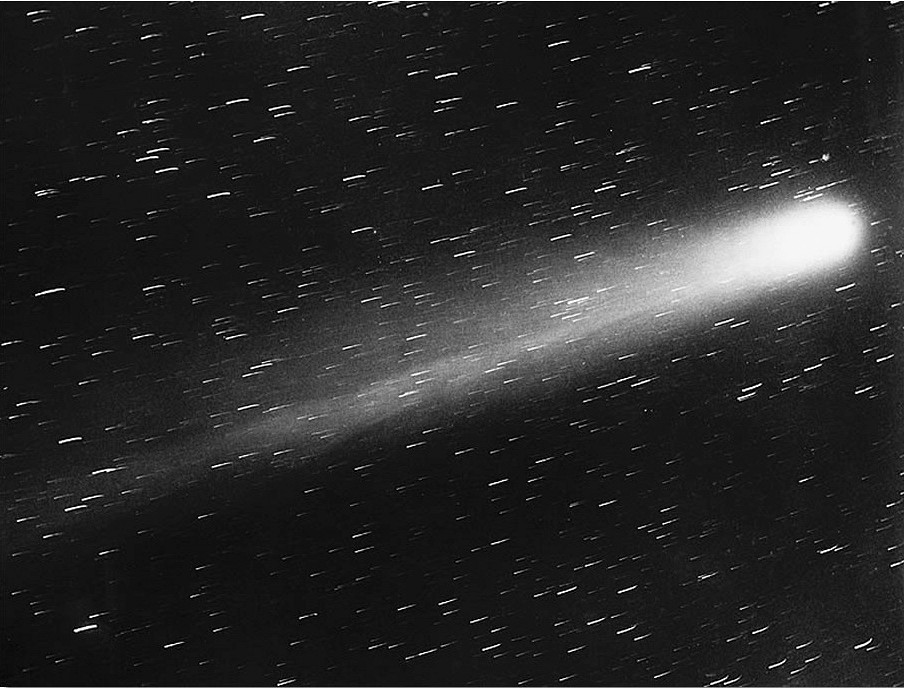
\includegraphics[width=\textwidth]{halley}}

\begin{document}

\begin{titlepage}
  \centering

  \makeatletter
  \vspace*{2cm}

  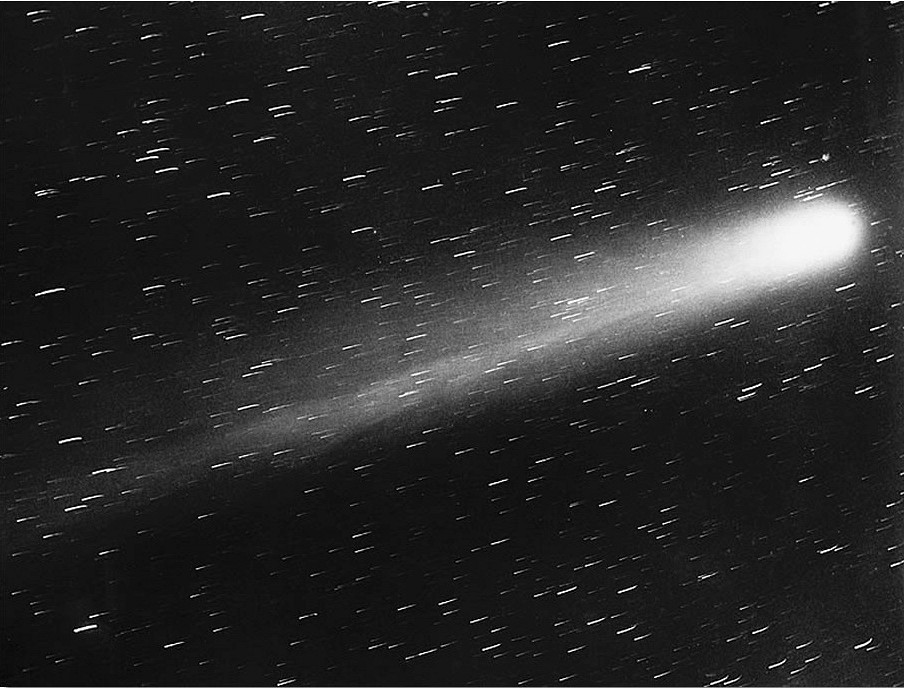
\includegraphics[width=\textwidth]{halley}

  \vspace*{\fill}

  \Huge{\textbf{\@title}}

  \vspace*{1cm}

  \Large\textit{\authors}

  \vspace*{\fill}

  \makeatother
\end{titlepage}

% \maketitle
\tableofcontents

\chapter*{Introduction}
This document is a brief overview of the topics in the NCEA L2 Physics
externals. There are some exercises, but it is designed to be read in
conjunction with a workbook or other source of problems (e.g. practice
exams).

\subsection*{Mathematical prerequisites}
It is assumed that all students are comfortable with mathematical concepts and skills equivalent to the standards
required for a merit or excellence level in the Level 1 Algebra standard. More precisely, you may wish to revise:
\begin{itemize}
  \item Solving linear equations.
  \item Basic trigonometry (triangle ratios and the Pythagorean theorem).
  \item Equations of parabolae and factoring quadratics.
  \item Knowledge of significant figures, scientific notation, and rounding.
\end{itemize}

However, this is above all a text on \textit{physics}; you need to be able to do simple calculations in the exam,
but the physical concepts and ideas are the main things which you should be aiming to learn.

\subsection*{A note about calculus}
Formally, calculus is not required for Level 2 Physics. However, an understanding of calculus roughly equivalent
to that in the L2 Calculus standard is useful for a deeper understanding of a few of the physics concepts that
we discuss this year (mainly in the mechanics standard).

\subsection*{Cover photo}
The cover photo to these notes depicts Halley's comet. This comet, which returns to the earth every 74-79 years, has been recorded
by astronomers since at least 240~BCE. It last passed the earth in 1986, and will next be seen in mid-2061.

\vspace*{\fill}
\begin{center}
  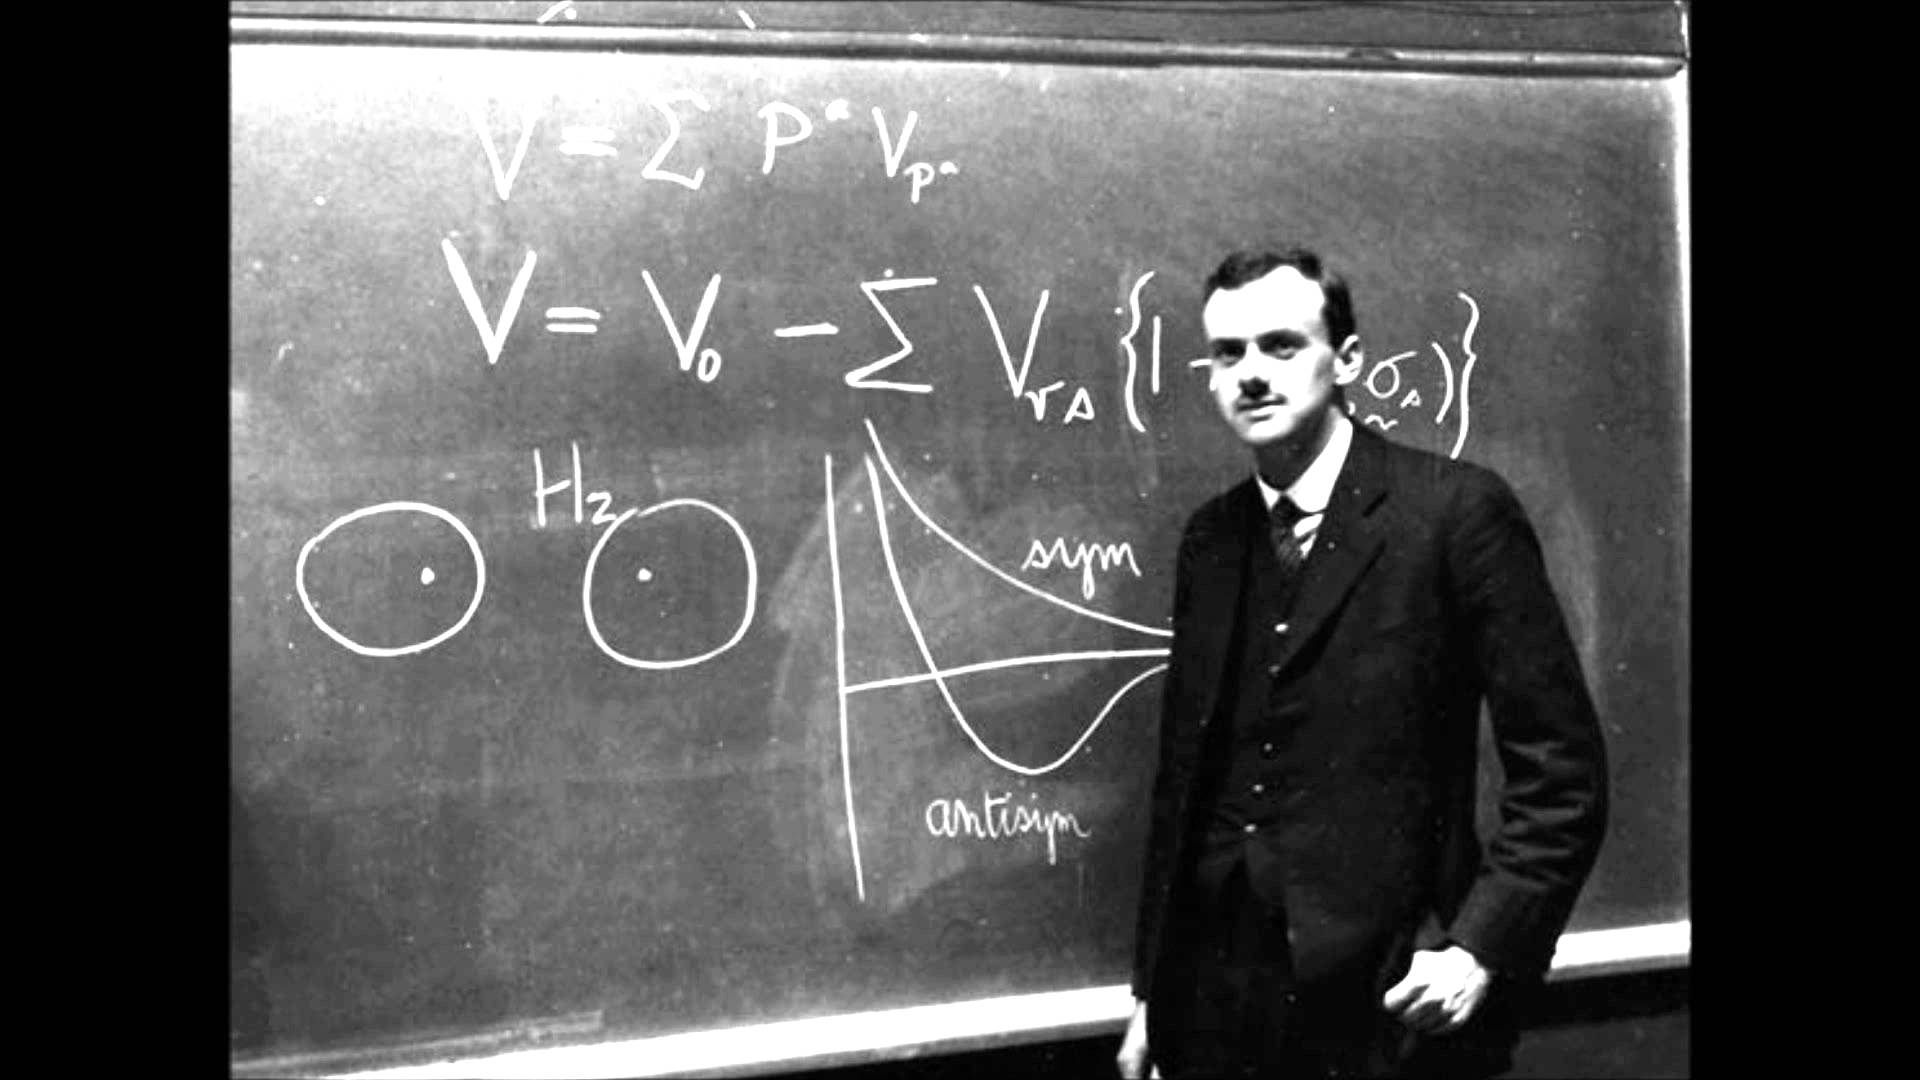
\includegraphics[width=0.85\textwidth]{dirac}\\
  \textit{I don't see how you can work on physics and write poetry at the same time. In science, you want to say
  something nobody know before, in words everyone can understand. In poetry, you are bound to say something that
  everybody knows already in words that nobody can understand.} - Paul Dirac
\end{center}

\chapter{91170: Demonstrate Understanding of Waves}
\section{What is a Wave?}
A wave, simply put, is a phenomenon by which energy is transferred from one location to another
without the movement of matter between the two locations. A wave is a periodic oscillation (repetition
of the same motion) in some medium (for example, water).

\subsection{Examples of Waves}
\begin{figure}
  \centering
  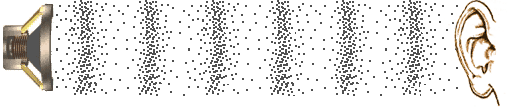
\includegraphics[width=\textwidth]{soundwave}
  \caption{The energy of a sound wave is carried by particles being compressed and then decompressed \capcite{http://www.mediacollege.com/audio/images/loudspeaker-waveform.gif}\label{fig:compwave}}
\end{figure}
\begin{figure}
  \centering
  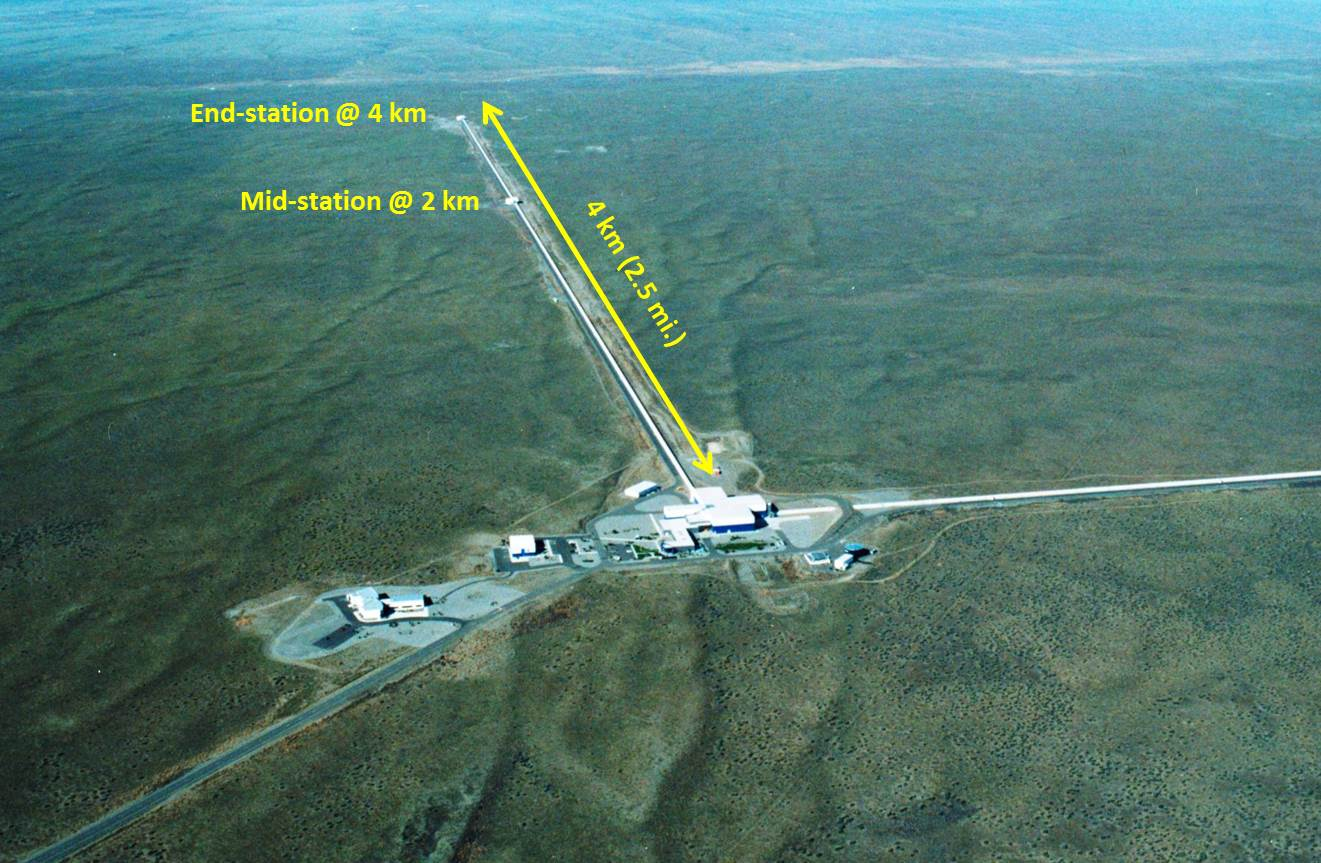
\includegraphics[width=\textwidth]{ligo}
  \caption{The LIGO project observed gravitational waves by measuring tiny changes in the length of their detector arm. \capcite{https://www.ligo.caltech.edu/system/media_files/binaries/271/original/Dual_detectors_with_arrow_and_stns_labeled.jpg?1453424757}\label{fig:ligo}}
\end{figure}
\begin{itemize}
  \item Waves in water are the movement of water molecules up and down while they remain in essentially the same position.
        The energy moves, but the net movement of water is zero (to a first approximation).
  \item Waves on a skipping rope are the movement of particles up and down --- the energy moves down the rope, but obviously
        the particles themselves cannot move down the rope!
  \item Sound waves are compression waves --- air particles move forwards and backwards in space, and the energy is transferred
        in the form of the compression fronts (figure \ref{fig:compwave}).
  \item Light can also be viewed as a wave; this time the wave is carried by vibrations in an invisible `electromagnetic field', similar
        to the gravitational field we are familiar with.
  \item Speaking of gravity, vibrations in a gravitational field called `gravitational waves' were observed in 2016 by LIGO (figure \ref{fig:ligo}).
\end{itemize}

\subsection{Classifying Waves}
\begin{figure}
  \centering
  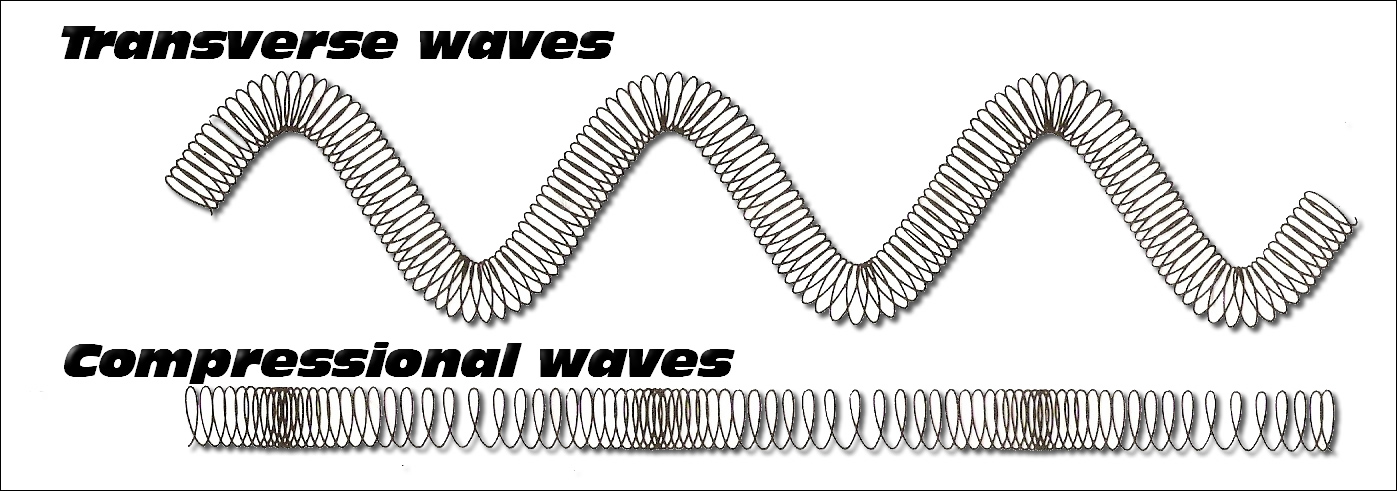
\includegraphics[width=\textwidth]{wavetypes}
  \caption{The two types of waves. \capcite{http://epiphanyvideoworks.com/Science/Hughes/Units/Energy/Energypictures/scan0010.jpg}\label{fig:wavetypes}}
\end{figure}
As seen above, there are in general two types of waves --- \textit{longitudinal (compression) waves}, in which the vibration of
the carrier particles occurs in the direction of wave propogation (e.g. sound waves and gravitational waves), and \textit{transverse waves},
in which particles oscillate up and down with respect to the wave direction. Figure \ref{fig:wavetypes} shows that both of these wave
types can be observed by oscillating a spring (or a slinky) in different ways.

\section{Reasoning Mathematically}
\begin{figure}
  \centering
  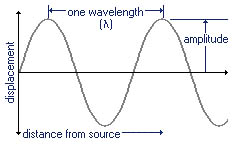
\includegraphics[width=0.5\textwidth]{sinewave}
  \caption{The parameters of a wave. \capcite{http://astro.uchicago.edu/cara/outreach/se/ysi/1999/diagram.jpg}\label{fig:sinewave}}
\end{figure}
We can view waves mathematically quite easily --- they can be modelled using sine and cosine curves. This year, however, we do not need
to go that deep into the mathematical theory; it is enough to be able to calculate some of the parameters of waves. It turns out that
to describe any wave, we only need to know the following values.

\subsection{The Parameters of a Wave}
See figure \ref{fig:sinewave}.
\begin{center}
\begin{tabularx}{\linewidth}{c|c|c|X}
  \textbf{Symbol} & \textbf{Name} & \textbf{Std. Unit} & \textbf{Description}\\\hline
  $ A $ & Amplitude & metre & The maximum displacement of a carrier particle from its rest position/the height of the crest above the zero position.\\
  $ \lambda $ (lambda) & Wavelength & metre & The distance between two successive corresponding positions (e.g. between crests).\\
  $ v $ & Velocity & \si{\metre\per\second} & The overall velocity of the wave-shape (remember that the average velocity of
                                              each \textbf{carrier particle} is zero).\\
  $ f $ & Frequency & \si{\hertz} (Hertz) & The number of waves passing a given point every second (\SI{1}{\hertz} is one wave per second).\\
  $ T $ & Period & second & The time taken for an entire wave to pass a point.
\end{tabularx}
\end{center}

\textit{The `energy content' of the wave is just the amplitude.}

You might also see \textit{wavenumber}: this is just $ \tilde\nu\text{ (nu)} = 1/\lambda $ (the number of wavefronts per metre, measured
in \si{\per\metre}). Sometimes $ \nu $ is also used to denote frequency (usually in chemistry).

\subsection{Relationships Between the Parameters}
First of all, note that the frequency is just the inverse of the period; in other words,
\begin{equation}
  f = \frac{1}{T}.
\end{equation}

Consider a set of waves travelling down a string. It takes a time $ T $ (where $ T $ is the period of vibration) for an entire
wavelength $ \lambda $ to pass a given point; hence the velocity of each wavefront is $ v = \frac{\Delta x}{\Delta t} = \frac{\lambda}{T} = f \lambda $.

This relation between velocity, frequency, and wavelength is known as the \textbf{fundamental wave equation}.
\begin{equation}
  v = f \lambda
\end{equation}

For an example, suppose you are sitting on a wharf and you count three waves hitting the wharf edge over one minute. Then
the period of the wave is $ 60/3 = \SI{20}{\second} $ (one wave takes a third of the time taken by three waves), and the
frequency is $ \frac{1}{20} = \SI{0.05}{\hertz} $. If you know that the wavelength (distance between successive wave crests)
is three metres, then the velocity of the wave must be $ v = f\lambda = 0.05 \times 3 = \SI{0.15}{\metre\per\second} $.

\subsection{Exercises}
\begin{enumerate}
  \item A sound wave travels at a speed of $ \SI{340}{\metre\per\second} $ in air. What wavelength does
        a note of frequency $ \SI{100}{\hertz} $ have?
  \item You notice that a given wave has crests hitting the shore on average every 30 seconds, and that the waves are coming into
        the shore at an average speed of \SI{0.5}{\metre\per\second}. What is the average distance between the wave crests?
\end{enumerate}

\section{Waves in Water}
\begin{figure}
  \centering
  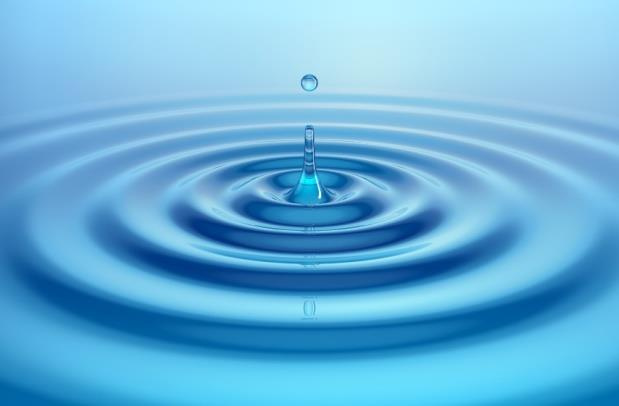
\includegraphics[width=0.5\textwidth]{pointsource}
  \caption{A circular wave generated by a point source (a dripping tap). \capcite{http://addins.wvva.com/blogs/weather/wp-content/uploads/2015/01/rippleinwater.jpg}\label{fig:pointsource}}
\end{figure}
\begin{figure}
  \centering
  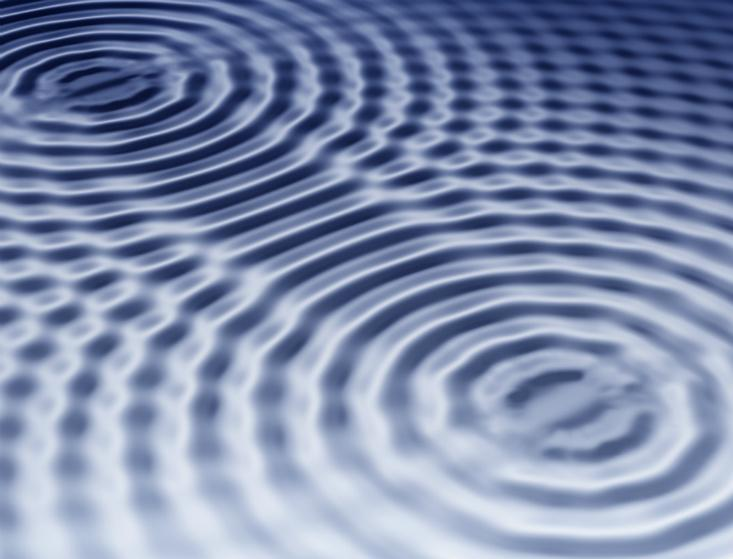
\includegraphics[width=0.5\textwidth]{pointsource2}
  \caption{The interference of two point sources. \capcite{http://static.nautil.us/2895_6b8b8e3bd6ad94b985c1b1f1b7a94cb2.jpg}\label{fig:pointsource2}}
\end{figure}
Let us consider qualitatively what happens to waves in water in several situations. First of all, we can generate
water waves in still water from a point source (as in figure \ref{fig:pointsource}) and then the waves radiate outwards in a circular
fashion. As the distance of the wavefront from the source becomes large, the wavefronts become nearly flat.

\subsection{Phase and Interference}
\begin{figure}
  \centering
  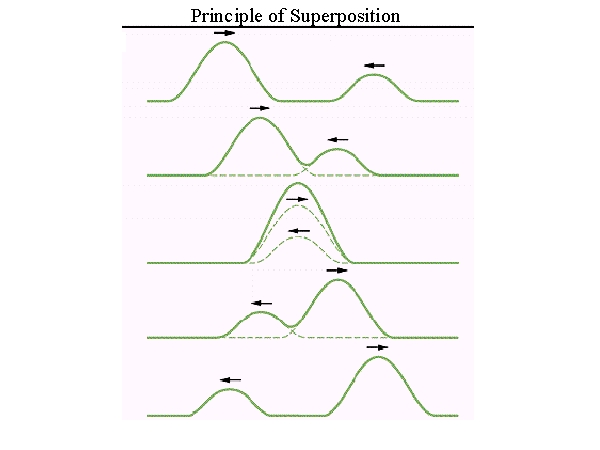
\includegraphics[width=0.7\textwidth]{superposition}
  \caption{The superposition of two waves. \capcite{http://www.cyberphysics.co.uk/topics/waves/img003.jpg}\label{fig:superposition}}
\end{figure}
\begin{figure}
  \centering
  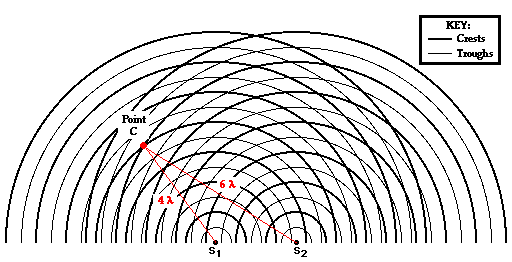
\includegraphics[width=0.9\textwidth]{pathdifference}
  \caption{The path difference here is $ 2\lambda $, and so constructive interference occurs. \capcite{http://www.physicsclassroom.com/Class/light/u12l3b3.gif}\label{fig:pathdifference}}
\end{figure}
\begin{figure}
  \centering
  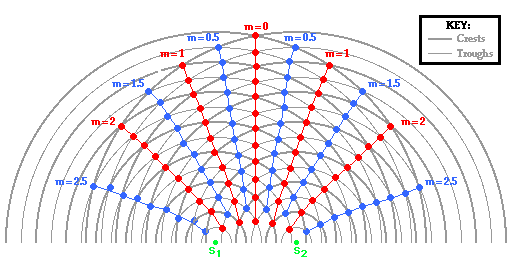
\includegraphics[width=0.9\textwidth]{pathdifference2}
  \caption{The red dots are the antinodes, and the blue dots are the nodes. Each $ m $ is the path difference of that line in multiples of the wavelength. \capcite{http://www.physicsclassroom.com/Class/light/u12l3b1.gif}\label{fig:pathdifference2}}
\end{figure}
Now, consider some point away from the point source. We call the `stage of the wave' that the point is going through the \textbf{phase} of
the wave at that point, and two points undergoing the same motion (for example, two crests) are said to be \textit{in phase}.
In general (for any wave), two points that are in phase are an exact number of wavelengths apart; two points undergoing exactly opposite
movement (e.g. a point at zero displacement and going down, and a point at zero displacement but going up) are said to be \textit{out of phase}
and are exactly an odd number of half-wavelengths apart.

If we place two identical point sources close to each other, as in figure \ref{fig:pointsource2}, we see areas where the waves meet and exactly cancel
each other out and the water does not move. This is because the two waves are cancelling each other out --- they are out of phase with each other at
that point. These points of \textit{total destructive interference} are called \textbf{nodes}, and they occur exactly where the difference between the
distances travelled by the waves from their respective sources (the path difference) is an odd number of half-wavelengths.

This suggests that when waves pass across each other, the net displacement at that point due to the \textbf{superposition} of the waves is just the sum
of the displacements of the individual waves --- when two waves are exactly out of phase, the displacement of one is the negative of the displacement
of the other and so the sum is zero. This intuitive idea is correct (figure \ref{fig:superposition}).

Going back to our double point-source example, if two waves are exactly in phase at some point (the path difference is a multiple of the wavelength, as
in figure \ref{fig:pathdifference}), total \textit{constructive interference} will occur - the amplitude of the wave at that point will be twice
the amplitude of one of the single point source waves. These points of \textit{maximum displacement} are called \textbf{antinodes}.

Figure \ref{fig:pathdifference2} summarises this.

\begin{center}
\begin{tcolorbox}[width=0.8\textwidth,colback={red},title={\textbf{Go and watch...}},colbacktitle=yellow,coltitle=blue]
  \textcolor{white}{\url{https://www.youtube.com/watch?v=J_xd9hUZ2AY}}
\end{tcolorbox}
\end{center}

\subsection{Reflection and Refraction}
\begin{figure}
  \centering
  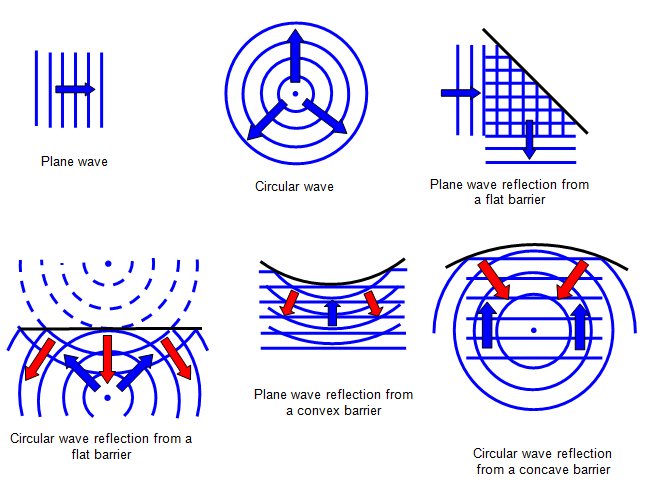
\includegraphics[width=0.9\textwidth]{waterreflect}
  \caption{The reflection of water waves. \capcite{http://www.schoolphysics.co.uk/age16-19/Wave\%20properties/Wave\%20properties/text/Wave_reflection_and_refraction/images/1.png}\label{fig:watreflect}}
\end{figure}
\begin{figure}
  \centering
  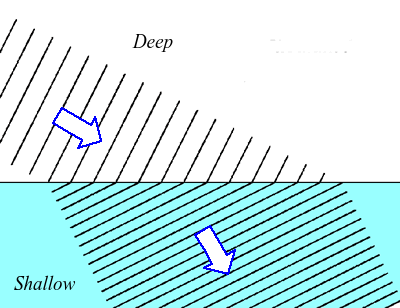
\includegraphics[width=0.5\textwidth]{refraction}
  \caption{The refraction of water waves. \capcite{http://www.school-for-champions.com/science/images/waves_obstacles_refraction.gif}\label{fig:refraction}}
\end{figure}
Let us now consider what happens when water waves hit a solid boundary, like a wall. We see that flat waves incident on a flat wall are reflected
at an angle (the angle of reflection) equal to the angle that they approach the wall at (the angle of incidence), but and that circular waves
on a flat wall are reflected in such a way that the individual rays of light are also reflected at the same angle that they are incident on
(see figure \ref{fig:watreflect}).

On the other hand, when flat waves approach a curved concave surface then the waves are all directed inwards to a single point (the focus)
and when flat waves approach a curved convex survace then the waves are all directed outwards away from a point inside the surface (again called
the focus).

When waves move across a boundary between deep and shallow water, as in figure \ref{fig:refraction} (where the blue area is shallower than the white area)
then they bend (one part of the wavefront slows down as it enters the shallow area first, but the rest of the wave continues on at the same speed).
When we move on to discussing light, we will develop this idea (known as \textbf{refraction}) mathematically.

\subsection{Diffraction}
\begin{figure}
  \centering
  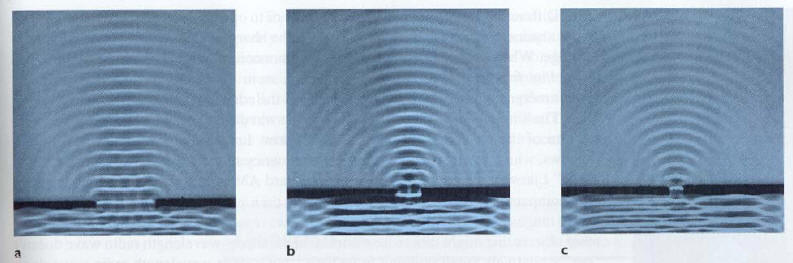
\includegraphics[width=\textwidth]{diffraction}
  \caption{The diffraction of water waves. \capcite{http://electron6.phys.utk.edu/light/images1-3/single1.jpg}\label{fig:diffraction}}
\end{figure}
\begin{figure}
  \centering
  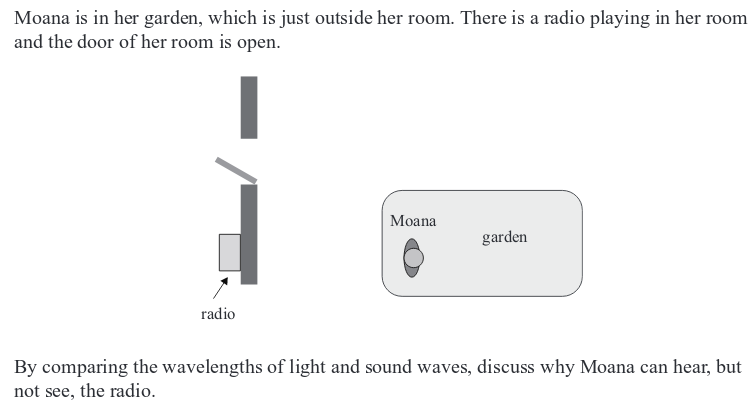
\includegraphics[width=\textwidth]{diffraction14}
  \caption{NZQA 91170 2014. \label{fig:diffraction-exam}}
\end{figure}
When water waves pass through a gap, they are compressed into a small width and then fan out again. This phenomenon, depicted in
figure \ref{fig:diffraction}, is known as \textbf{diffraction}. The angle of the fanning depends on the ratio between the width of the
gap and the wavelength; if the wavelength is large compared to the width of the gap, then the diffraction effect is much more pronounced
than if the wavelength is small compared to the width of the gap.

Consider the question given in figure \ref{fig:diffraction-exam}. This is an excellent illustration of the kind of thing we can explain using
the phenomenon which we discuss in the waves standard: sound waves have a much higher wavelength than the light waves and so diffract
much more (the diffraction of the light is negligible), which is why we can hear around corners but not see around them.

\begin{center}
\begin{tcolorbox}[width=0.8\textwidth,colback={red},title={\textbf{Go and watch...}},colbacktitle=yellow,coltitle=blue]
  \textcolor{white}{\url{https://www.youtube.com/watch?v=2TMR-EyF_ds}}
\end{tcolorbox}
\end{center}

\section{Pulses in a String}
\begin{figure}
  \centering
  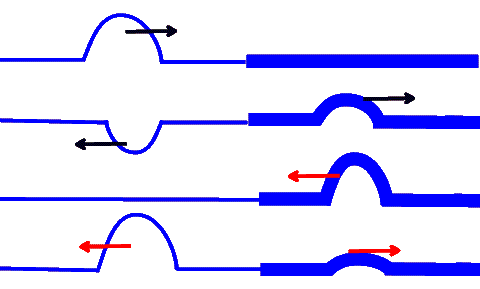
\includegraphics[width=0.7\textwidth]{string}
  \caption{Pulse transmission in a string. \capcite{http://minerva.union.edu/newmanj/physics100/light\%20as\%20a\%20wave/outofphasewaves.gif}\label{fig:string}}
\end{figure}
Suppose we have a string made up of two parts, one light section and one heavy section. If we send a pulse from the light section
into the heavy section, we find that some of the energy is transmitted across the \textbf{medium boundary}, but that some of the
energy is also reflected (in such a way that the wave becomes inverted). A similar phenomenon occurs if the wave moves from the
heavy to the light string. Both situations are summarised in figure \ref{fig:string}.

We also note that the wave on the heavy string moves slower than that on the light string; the amplitudes of the reflected and transmitted
waves are less than the original amplitude, due to conservation of energy.

When we move to discuss light, this idea of reflection and transmission across a wave boundary will become incredibly important;
for example, it allows us to explain how you can look at a swimming pool and see both swimmers within the water and your own reflection
at the same time.

\section{What About Light?}
\begin{figure}
  \centering
  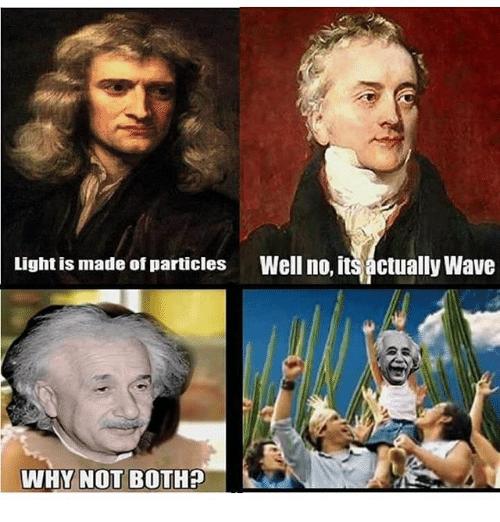
\includegraphics[width=0.7\textwidth]{lightisweird}
  \caption{Light is weird. \capcite{https://pics.onsizzle.com/Instagram-109383.png}\label{fig:lightisweird}}
\end{figure}
Is light a particle or a wave? Well, this is not a question we can answer this year and so we avoid the question by noticing that this
is the wave standard, and so we will treat it as a wave here and see how far we get. We can apply everything we've already done to predict
how light should behave:
\begin{itemize}
  \item It should interfere with itself.
  \item It should reflect off stuff.
  \item It should be able to refract through medium boundaries.
  \item It should diffract through tiny gaps.
\end{itemize}

We will also introduce some mathematical analysis which we glossed over when discussing water waves --- the analysis
done here will work for \textbf{all waves}.

Firstly, here are some properties of light which will be useful:
\begin{itemize}
  \item Light always travels in straight lines (over short distances, anyway: it turns out that light from distant stars is actually bent
        by gravity! The stars are not where we see them because of this effect.)
  \item The speed of light in a vacuum is \SI{2.99e8}{\metre\per\second}, but it slows down in some mediums (the speed of
        light in glass is around \SI{1.99e8}{\metre\per\second}).
  \item Light carries energy (obviously: the sun heats the earth!)
  \item All electro-magnetic radiation is a light wave (e.g. radiowaves and microwaves, as well as gamma rays).
  \item The range of wavelengths of visible light is around \SI{390}{\nano\metre} (violet) to \SI{700}{\nano\metre} (red).
  \item Illumination of a point follows the inverse square law (i.e. if a point is a distance $ d $ away from a light source,
        the illumination is $ I \propto \frac{1}{d^2} $).
\end{itemize}

\begin{figure}
  \centering
  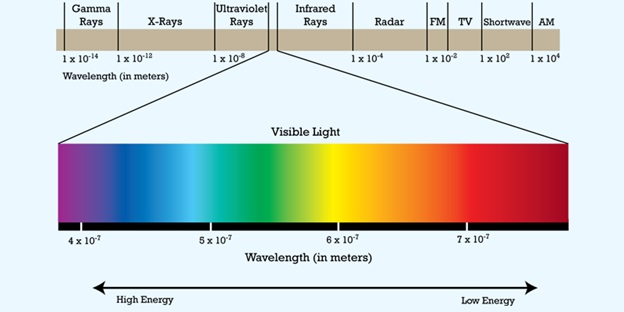
\includegraphics[width=\textwidth]{visible-light-1}
  \caption{The various kinds of EM radiation (light waves) \capcite{http://byjus.com/physics/wp-content/uploads/2016/06/Visible-light-1.jpg}\label{fig:visible}}
\end{figure}

\subsection{The Double-Slit Experiment}
\begin{figure}
  \centering
  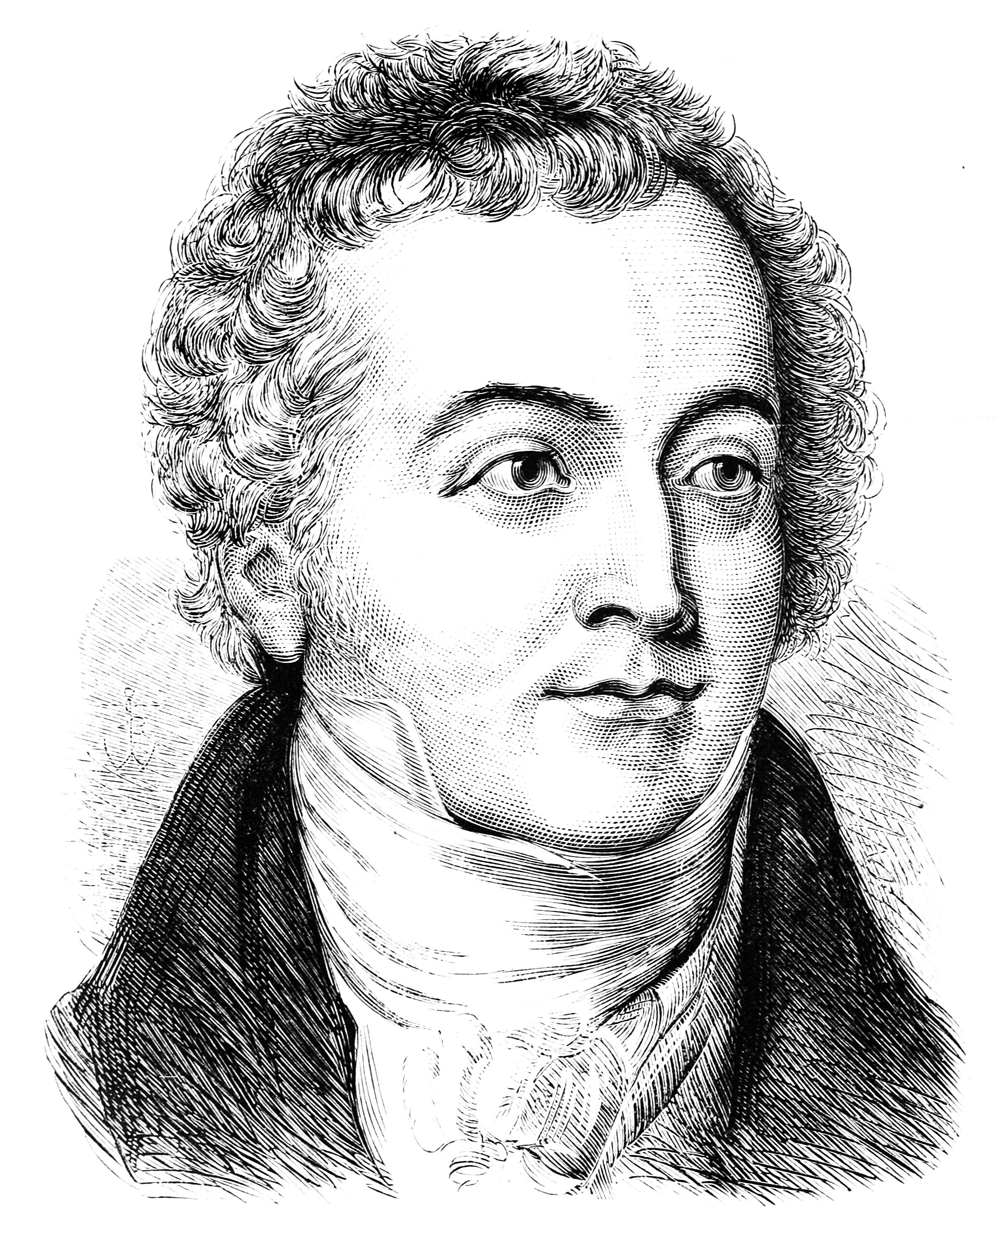
\includegraphics[width=0.3\textwidth]{young}
  \caption{Thomas Young.\label{fig:young}}
\end{figure}
\begin{figure}
  \centering
  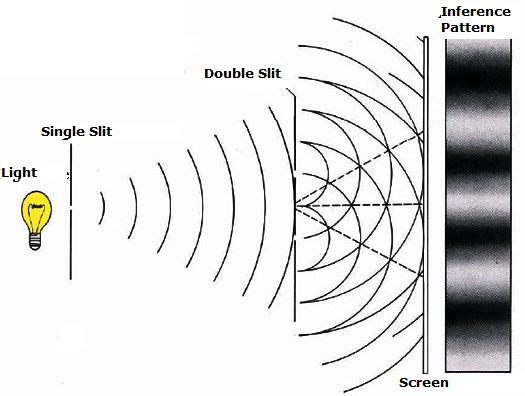
\includegraphics[width=0.7\textwidth]{doubleslit}
  \caption{Young's double-slit experiment.\label{fig:doubleslit}}
\end{figure}
If we pass light through two small gaps close to each other (around \SI{0.1}{\milli\metre} apart), we essentially create two
in-phase point sources. We can project the resulting wave onto a screen, and we observe the interference pattern seen in
figure \ref{fig:doubleslit}. This experiment was first performed by Thomas Young (figure \ref{fig:young}) in 1801, and exhibits
both the diffraction and interference of light --- the bright patches are areas of total constructive interference, and the
dark patches are regions of total destructive interference. Next year, we will analyse this two dimensional case mathematically,
and we will be able to calculate the locations of the observed fringes.

If we use two \textbf{independent} sources (e.g. two bulbs rather than one) then no interference pattern is seen due to the point
sources being randomly out-of-phase --- in this situation, the two sources are called \textit{incoherent}.

\subsection{Reflection}
\begin{figure}
  \centering
  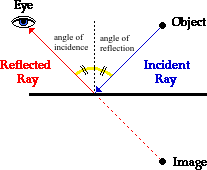
\includegraphics[width=0.5\textwidth]{reflection}
  \caption{The reflection of light in a flat mirror \capcite{http://www.physicsclassroom.com/Class/refln/u13l1c2.gif}\label{fig:reflection}}
\end{figure}
Reflection can be observed in two ways:
\begin{itemize}
  \item Perfect mirrors reflect all light.
  \item Objects reflect only some wavelengths (how we see).
\end{itemize}
We will only describe perfect reflection this year, as it is much easier to analyse.

When light is incident (falls onto) a flat mirror (a \textbf{plane mirror}), the angle of reflection is always equal to the angle
of incidence. This result is the \textit{fundamental result} of reflection and is the \textbf{key idea} which allows us to analyse
reflection of all waves.

Note that the brain is stupid --- it thinks that light always travels in straight lines, and so it sees the image as
being \textit{inside the mirror}. This is known as a \textit{virtual image}, since there are no actual light rays at
the position of the image (only imagined ones).

In a plane mirror, the distance of the image from the mirror is equal to the distance of the object from the mirror; the size
of the image is also equal to the size of the object.

\begin{figure}
  \centering
  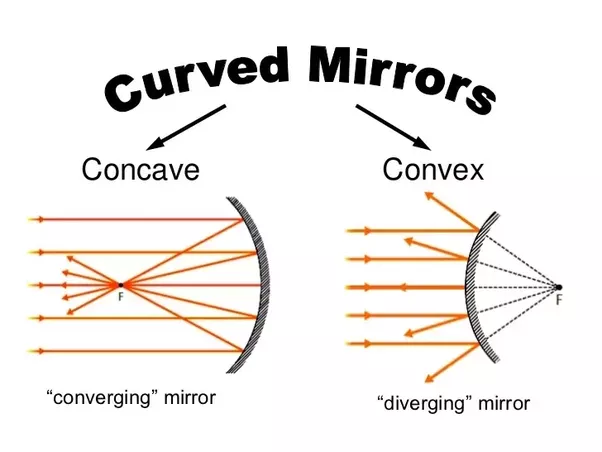
\includegraphics[width=0.5\textwidth]{curved}
  \caption{The reflection of light in a curved mirror\\ \capcite{https://qph.ec.quoracdn.net/main-qimg-c84654e146945deec5ee6491cb547873}\label{fig:curved}}
\end{figure}

Now, suppose we take a section of a sphere and make it reflective. If the inside is reflective, the mirror is known as \textit{concave};
if the outside is reflective, the mirror is known as \textit{convex}. Both of these are shown in figure \ref{fig:curved}. The \textit{focus}
of the mirror is an important point as it determines where light rays are reflected to. The \textit{radius of curvature} of a spherical
mirror is twice the focal length (distance from focus to mirror).

\begin{center}
\begin{tcolorbox}[width=0.8\textwidth,colback={red},title={\textbf{Go and watch...}},colbacktitle=yellow,coltitle=blue]
  \textcolor{white}{\url{https://www.youtube.com/watch?v=zRP82omMX0g}}
\end{tcolorbox}
\end{center}

\begin{figure}
  \centering
  \begin{subfigure}[t]{0.5\textwidth}
    \centering
    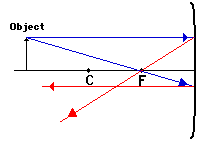
\includegraphics[width=.8\linewidth]{concave}
    \caption{Concave\\ \capcite{http://www.physicsclassroom.com/Class/refln/u13l3d2.gif}\label{fig:concave}}
  \end{subfigure}%
  \begin{subfigure}[t]{0.5\textwidth}
    \centering
    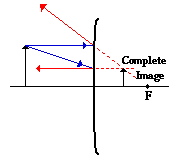
\includegraphics[width=.8\linewidth]{convex}
    \caption{Convex\\ \capcite{http://www.physicsclassroom.com/Class/refln/u13l4b4.gif}\label{fig:convex}}
  \end{subfigure}
  \caption{Ray diagrams for curved mirrors.}
\end{figure}

We first consider a concave mirror. Rays of light incident directly onto the mirror parallel to the principle axis (joining the focus
to the centre of the mirror) are reflected through the focus, and rays through the focus are reflected directly out. The image appears
where the light rays from the object converge for the second time --- for example, if the object is outside the focus then the diagram
will look like figure \ref{fig:concave}. In the figure, the image formed is inverted, smaller than the object, and real --- although if
the object is closer to the mirror than the focus $ F $, the image formed is virtual.

The same rules apply for a convex mirror, only this time light rays are reflected away from the focus if they come in straight and are
reflected straight if they come in on a line to the focus (figure \ref{fig:convex}). Convex mirrors always produce virtual images that
are upright and smaller than the object.

If $ D_o $ is the distance from the mirror to the object, and $ D_i $ is the distance from the mirror to the image, then
the two are related by Descartes' formula:
\begin{equation}
  \frac{1}{f} = \frac{1}{D_o} + \frac{1}{D_i}
\end{equation}
The heights of the image and object can also be related:
\begin{equation}
  \text{magnification} = m = \frac{D_i}{D_o} = \frac{H_i}{H_o}
\end{equation}

When using these formulae, be careful: if a distance is \textbf{virtual} (behind the mirror), it is always negative. This means
that:
\begin{itemize}
  \item If the image is formed behind the mirror, $ D_i $ is negative.
  \item A virtual image has a negative height $ H_i $.
  \item The focal length of a \textbf{convex} mirror is negative.
\end{itemize}

\paragraph{Example.} How far should an object be placed in front of a concave spherical miror, with a radius
of curvature of \SI{36}{\centi\metre}, to form a real image $\frac{1}{9}$ of its size?

We have $ f = 36/2 = 18 $, and $ H_i = \frac{1}{9} H_o $. But $ D_i/D_o = H_i/H_o $, so $ D_i = \frac{D_o}{9} $.
Hence applying Descartes' Formula:
\begin{displaymath}
  \frac{1}{f} = \frac{1}{D_i} + \frac{1}{D_o} \Rightarrow \frac{1}{18} = \frac{9}{D_o} + \frac{1}{D_o} = \frac{10}{D_o}
\end{displaymath}
and therefore $ D_o = \SI{180}{\centi\metre} $.

\paragraph{Exercise.} An object \SI{2}{\centi\metre} high is placed \SI{12}{\centi\metre} in front of a concave
mirror of focal length \SI{4}{\centi\metre}. Draw a ray diagram, and calculate the position and height of the
image formed.

\paragraph{Exercise.} It is possible to form an image with a magnification of 2 when the object is \SI{12}{\centi\metre}
from a mirror. Find the focal length of the mirror if the image is virtual.

\subsection{Refraction}
\begin{figure}
  \centering
  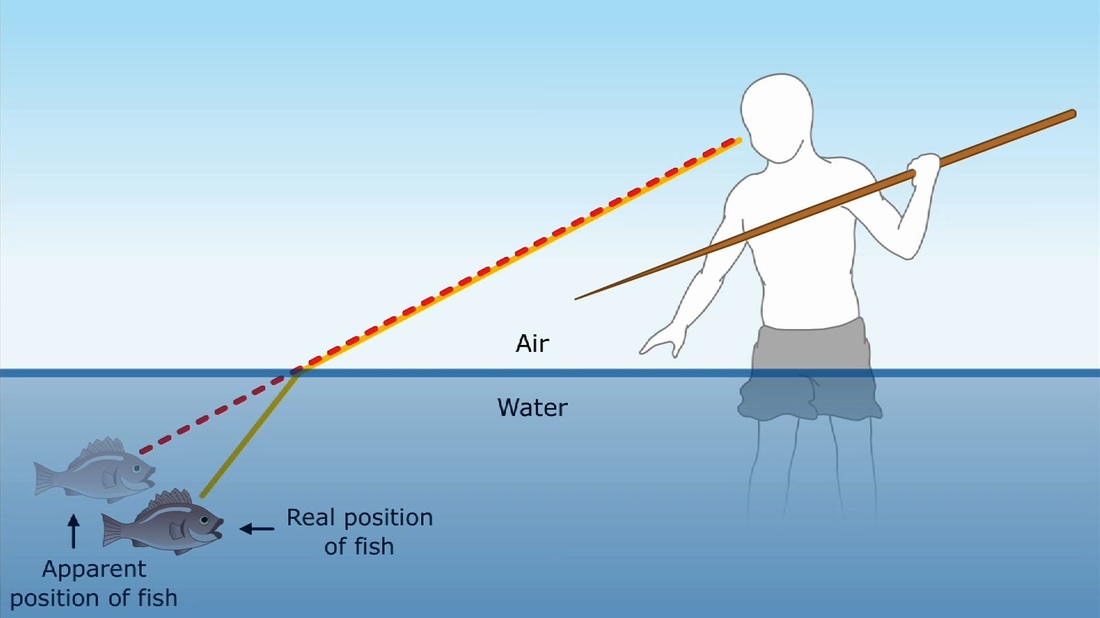
\includegraphics[width=\textwidth]{lightrefraction}
  \caption{The refraction of light as it passes across a medium boundary \capcite{http://munnscience.weebly.com/uploads/3/8/0/6/38066171/158235059.jpg}\label{fig:lightrefracts}}
\end{figure}
When we looked at waves on string, we observed that when waves move from one medium to another their speed changed. We observed
the same thing with water waves, when they moved from deep water to shallow water. The same effect occurs with light when it
crosses a medium boundary (as in figure \ref{fig:lightrefracts}).

\begin{center}
\begin{tcolorbox}[width=0.8\textwidth,colback={red},title={\textbf{Go and watch...}},colbacktitle=yellow,coltitle=blue]
  \textcolor{white}{\url{https://www.youtube.com/watch?v=Bf1k9-4bb4w}}
\end{tcolorbox}
\end{center}

We have already observed that this refraction is becase part of the light wavefront slows down before the rest; we now analyse
this mathematically. First, note that the frequency of the light cannot change as it crosses a medium boundary. Hence, we
can write down the following relationship between the wavelengths and velocities:
\begin{displaymath}
  \frac{\lambda_1}{\lambda_2} = \frac{v_1}{v_2}
\end{displaymath}

\begin{figure}
  \centering
  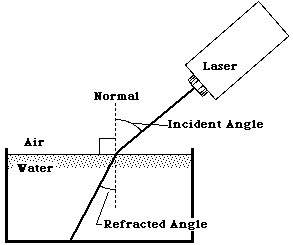
\includegraphics[width=0.7\textwidth]{refractionangle}
  \caption{The refraction of light when it moves from air to water, with angles shown. \capcite{http://www.cbakken.net/obookshelf/image027.gif}\label{fig:refractionangles}}
\end{figure}

We can even relate the angle of incidence $ \theta_1 $ and the angle of refraction $ \theta_2 $ (see figure \ref{fig:refractionangles}) as
follows:
\begin{displaymath}
  \frac{\lambda_1}{\lambda_2} = \frac{v_1}{v_2} = \frac{\sin \theta_1}{\sin \theta_2}
\end{displaymath}

\paragraph{Exercise.} Explain why a straw sitting in a glass of clear water appears bent when we look at.

\paragraph{Exercise.} Explain why we can see beads of water on a glass window even though both are transparent.

\begin{center}
\begin{tcolorbox}[width=0.8\textwidth,colback={red},title={\textbf{Go and watch...}},colbacktitle=yellow,coltitle=blue]
  \textcolor{white}{\url{https://www.youtube.com/watch?v=_1plSYKR7Oo}}
\end{tcolorbox}
\end{center}

Earlier, I mentioned that the speed of light changes when it enters a medium. Let $ c $ be the speed of
light in a vacuum, and let $ v_m $ be the speed of light in some medium; then we define
\begin{equation}
  n_m = \frac{c}{v_m}
\end{equation}
to be the \textbf{absolute refractive index}, or the \textbf{optical density} of the medium.

It turns out that when light travels from one medium with a refractive index $ n_1 $
to another with refractive index $ n_2 $ then (note the swapped subscripts):
\begin{displaymath}
  _1 n_2 = \frac{n_2}{n_1} = \frac{v_1}{v_2}
\end{displaymath}
This number $ _1 n _2 $ is called the \textbf{relative refractive index}.

Hence we have the fundamental equation of refraction:
\begin{equation}
  _1 n _2 = \frac{n_2}{n_1} = \frac{\lambda_1}{\lambda_2} = \frac{v_1}{v_2} = \frac{\sin \theta_1}{\sin \theta_2}
\end{equation}

It is often much easier to remember that $ n_1 \sin \theta_1 = n_2 \sin \theta_2 $ (Snell's Law).

\begin{center}
\begin{tabular}{c|c||c|c}
  \textbf{Substance} & $ n $ & \textbf{Substance} & $ n $\\\hline
  Diamond & 2.42 & Perspex & 1.49\\ 
  Ruby & 1.76 & Paraffin Oil & 1.44\\
  Flint Glass & 1.65 & Ethanol & 1.36\\
  Crown Glass & 1.52 & Water & 1.33\\
  NaCl & 1.53 & Ice & 1.31\\
  Benzene & 1.50 & Air & 1.0003\\
\end{tabular}
\end{center}

\paragraph{Exercise.} For a light ray passing from glass ($ n_1 = 1.52 $) to water ($ n_2 = 1.33 $), find the angle
of refraction if the angle of incidence is \SI{35}{\degree}.

\paragraph{Exercise.} Find the speed of light in benzene.

\subsection{Total Internal Reflection}
\begin{figure}
  \centering
  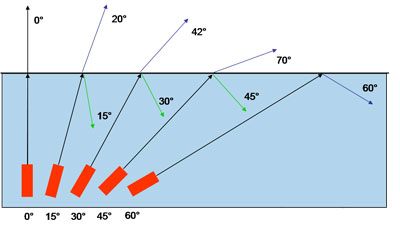
\includegraphics[width=0.7\textwidth]{criticalangle}
  \caption{An example of total internal reflection. \capcite{http://www.timbercon.com/assets/Uploads/fiber-optic-glossary/images/Critical-Angle.jpg}\label{fig:tire}}
\end{figure}
Like with strings, not all the light is refracted when we pass a medium boundary --- some light is reflected back into
the medium (like looking up at the surface of the water when diving).

When light travels from one medium to another that is less optically dense (i.e. has a lower refractive index --- like from glass to air),
the angle of incidence is less than the angle of refraction (the light bends away from the normal). It is therefore possible to, at some
angle of incidence, to have an angle of refraction of \SI{90}{\degree}. This angle of incidence is known as the \textit{critical angle}
of the medium. If we exceed the critical angle, then \textit{no refraction occurs} --- all the light incident on the boundary is \textit{totally
reflected back into the first medium}. This phenomenon is known as \textit{total internal reflection}.

The two conditions for total internal reflection to occur are:
\begin{itemize}
  \item Light passes from a higher optical density medium to a lower optical density medium (i.e. $ n_2 < n_1 $), and
  \item The angle of incidence $ \theta_1 $ is greater than the critical angle $ \theta_c $.
\end{itemize}

See figure \ref{fig:tire}, which shows a critical angle of \SI{60}{\degree}.

One pretty example of total internal reflection is the sparkling of diamond; due to the high refractive index of a diamond,
a beam of light can be trapped inside the crystal and be emitted in a random direction when it emerges. Total internal reflection
is also the phenomenon behind fibre optic cables.

\subsection{Prisms}
\begin{figure}
  \centering
  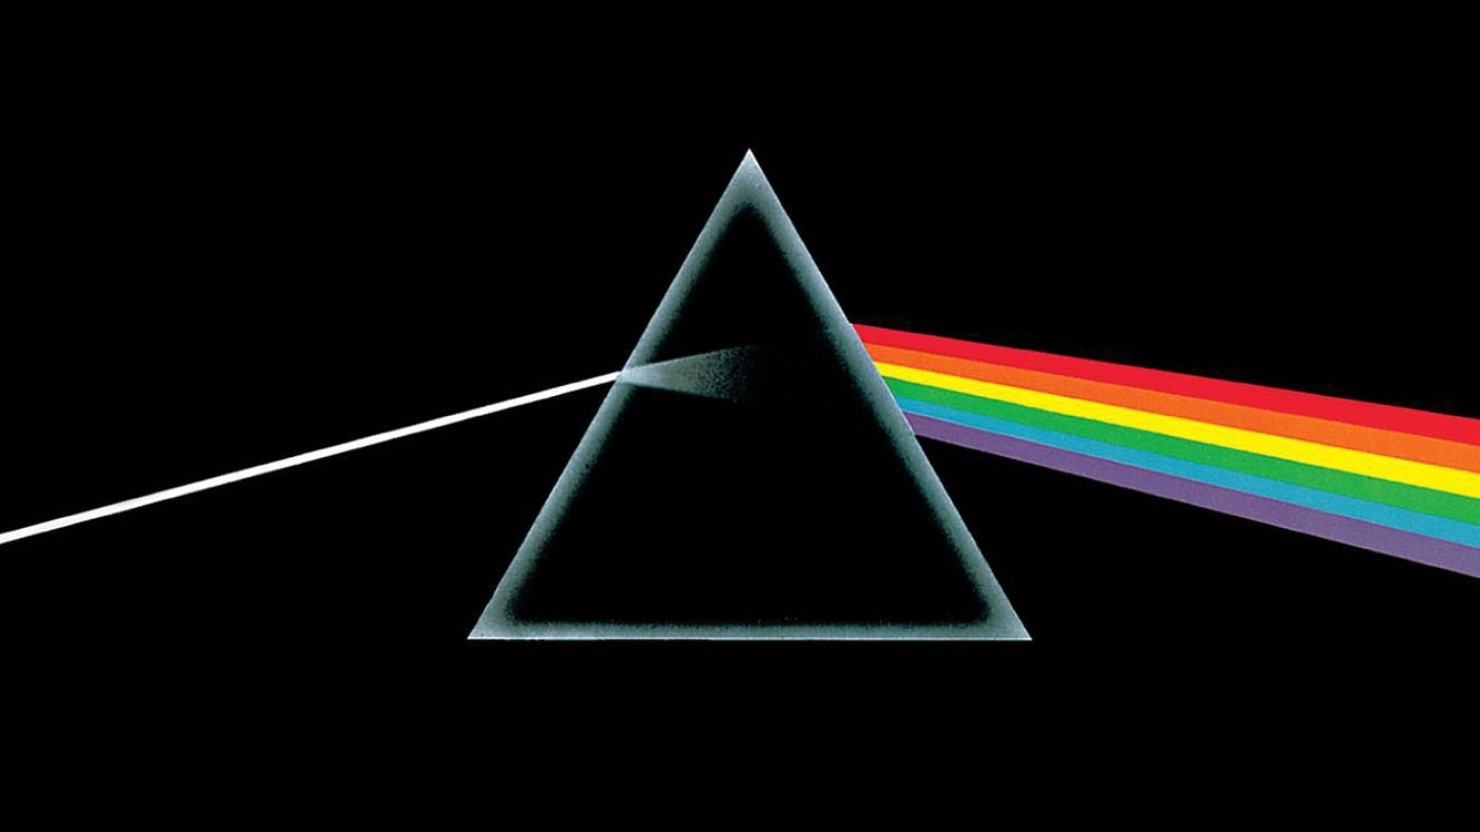
\includegraphics[width=0.7\textwidth]{prism}
  \caption{Refraction of white light through a prism. \capcite{https://www.jambase.com/wp-content/uploads/2016/03/DSOTM-Crop-1480x832.jpg}\label{fig:prism}}
\end{figure}
The angle of refraction depends on the frequency of light; hence when we pass white light through a prism, the different frequencies
of light split apart (they are bent at different angles), as in figure \ref{fig:prism}. Violet light has the highest frequency of all the visible
colours and so is refracted the most; red light has the lowest frequency and so is refracted the least (see figure \ref{fig:visible}).

\subsection{Lenses}
\begin{figure}
  \centering
  \begin{subfigure}[t]{0.5\textwidth}
    \centering
    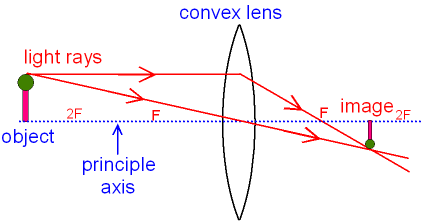
\includegraphics[width=.8\linewidth]{lense1}
    \caption{Convex lens ($D_o > f $).\\ \tiny{\capcite{http://www.gcsescience.com/convex-lens-image-real-inverted-smaller.gif}}\label{fig:lens1}}
  \end{subfigure}%
  \begin{subfigure}[t]{0.5\textwidth}
    \centering
    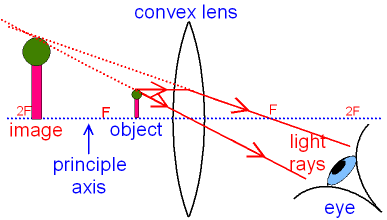
\includegraphics[width=.8\linewidth]{lense2}
    \caption{Convex lens ($D_o < f $).\\ \tiny{\capcite{http://www.gcsescience.com/convex-lens-magnifying-glass.gif}}\label{fig:lens2}}
  \end{subfigure}
  \begin{subfigure}[t]{0.5\textwidth}
    \centering
    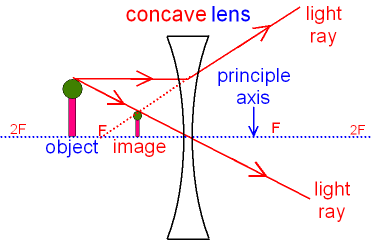
\includegraphics[width=.8\linewidth]{lense3}
    \caption{Concave lens.\\ \tiny{\capcite{http://www.gcsescience.com/concave-lens-ray-diagram-divergent.gif}}\label{fig:lens3}}
  \end{subfigure}
  \caption{Ray diagrams for lenses.\label{fig:lenses}}
\end{figure}
Lenses are easy! They work in exactly the same way as mirrors (well, sort of). Convex lenses cause parallel light rays to
converge at the focus, while concave lenses cause parallel light rays to diverge away from the focus. See the ray diagrams
in figure \ref{fig:lenses}. Note that each lens has \textbf{two} equidistant focii. Descartes' formula also works for lenses:

\paragraph{Example.} Find the position and magnification of an image formed by a convex lens of focal length \SI{100}{\centi\metre}
when the object is \SI{150}{\centi\metre} from the lens.

\begin{displaymath}
  \frac{1}{100} = \frac{1}{150} + \frac{1}{D_i} \Rightarrow \frac{1}{D_i} = \frac{1}{300}
\end{displaymath}
So the object is \SI{300}{\centi\metre} from the lens (on the other side). The magnification is $ m = \frac{D_i}{D_o} = \frac{300}{150} = 2 $.

\chapter{91171: Demonstrate Understanding of Mechanics}
\section{Vectors and Scalars}
When we talk about the motion of an object, it is often important to mention the direction of movement as well as the
rate. When we include a direction with a number, the resultant quantity is called a \textit{vector}. A number by itself,
in contrast, is called a \textit{scalar}.

\begin{center}
\begin{tcolorbox}[width=0.8\textwidth,colback={red},title={\textbf{Go and watch...}},colbacktitle=yellow,coltitle=blue]
  \textcolor{white}{\url{https://www.youtube.com/watch?v=V8hJhTE3bUk}}
\end{tcolorbox}
\end{center}

\subsection{Examples of vector quantities}
\begin{figure}
  \centering
  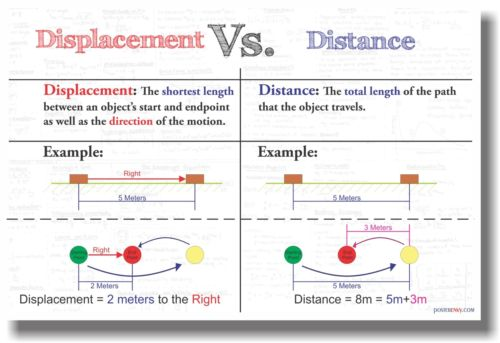
\includegraphics[width=0.7\textwidth]{displacement}
  \caption{The difference between displacement and distance.\label{fig:displacement}}
\end{figure}

\begin{center}
\begin{tabular}{c|c}
  \textbf{Scalar} & \textbf{Vector}\\\hline
  Distance & Displacement\\
  Speed & Velocity\\
  & Acceleration\\
  Energy &\\
  Mass &\\
  & Momentum\\
  & Force\\
  Area (well...) &\\
  Work &\\
  Power &\\
  Density &\\
  Pressure &\\
  Time &
\end{tabular}
\end{center}

Vectors can be given either by the coordinates of their endpoints, or by a length (magnitude) and angle from the positive $ x$-axis.

\begin{figure}
  \centering
  
\includegraphics[width=0.4\textwidth]{dunne}
  \caption{The former Peter Dunne.\label{fig:dunne}}
\end{figure}

\paragraph{Exercise.} An electoral candidate, newly hopeful due to the resignation of Peter Dunne (figure \ref{fig:dunne}), travels around Wellington. They
began by travelling \SI{5.0}{\kilo\metre} east, then \SI{3.0}{\kilo\metre} north, then \SI{4.0}{\kilo\metre} west, and finally \SI{2.0}{\kilo\metre}
south. What is their final displacement from their starting point (in terms of the distance and angle from the east axis)?

\subsection{Adding and Subtracting Vectors}
\begin{figure}
  \centering
  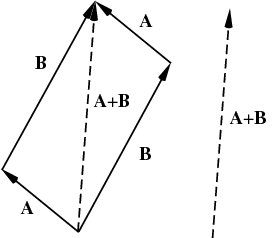
\includegraphics[width=0.5\textwidth]{parallelogram}
  \caption{The parallelogram rule for adding vectors. \capcite{http://mathworld.wolfram.com/images/eps-gif/ParallelogramLaw_1000.gif}\label{fig:parallelogram}}
\end{figure}
Later on, it will be important to be able to add and subtract vectors. Luckily, it's quite
simple: you simply place the vector arrows end-to-end and the new endpoint is the end of
your new vector (figure \ref{fig:parallelogram}).

If we multiply a vector by a scalar, we simply scale the length of the vector by the amount
specified --- if $ \vec v $ is a vector, then $ 2 \vec v $ has the same direction but twice the length.

The subtraction $ \vec v - \vec w $ is simply defined to be $ \vec v + (- \vec w) $, where $ - \vec w $ is the vector with
the same length as $ \vec w $ but the opposite direction.

\section{Linear Motion}
Suppose a car is travelling in a straight line and covers \SI{2}{\metre} every second. We call this
ratio the \textit{speed} of the car; the \textit{velocity} of the car is simply the speed together
with the direction. By definition, if a car travels a displacement $ \Delta \vec s $ over a length of time $ \Delta t $
then we have
\begin{equation}
  \vec v = \frac{\Delta \vec s}{\Delta t} = \od{\vec s}{t}
\end{equation}
\textbf{Velocity is the rate of change of displacement with respect to time.}

Similarly, we define the \textbf{acceleration} of an object to be the rate of change of \textit{velocity} with
respect to time:
\begin{equation}
  \vec a = \frac{\Delta \vec v}{\Delta t} = \od{\vec v}{t}
\end{equation}

Since velocity is a vector, the an object changes when its direction of motion changes even if its
speed remains constant.

\subsection{Graphing Motion}
\begin{figure}
  \centering
  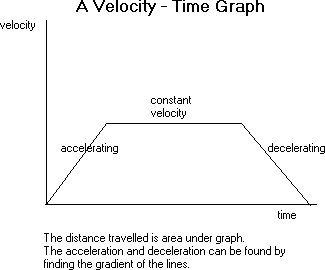
\includegraphics[width=0.6\textwidth]{vgraph}
  \caption{A velocity-time graph. \capcite{https://revisionworld.com/sites/revisionworld.com/files/imce/travelgraph2.gif}\label{fig:vgraph}}
\end{figure}
When we graph displacement against time:
\begin{itemize}
  \item The slope of the graph at a point is the speed at that time (this is the derivative).
\end{itemize}

When we graph instantaneous velocity against time (figure \ref{fig:vgraph}):
\begin{itemize}
  \item The slope of the graph at a point is the acceleration at that time (this is the derivative).
  \item The area under the curve between two points is the displacement between those points (this is the integral).
\end{itemize}

When we graph instantaneous acceleration against time:
\begin{itemize}
  \item The area under the curve between two points is the average velocity between those points (this is the integral).
\end{itemize}

\subsection{Kinematic Equations}
We will drop the vector symbols from now on for convenience. Suppose the acceleration $ a $ of a particle is
constant over some time interval $ t $, that its displacement over that time is $ d $, and that its final and
initial velocities are $ v_f $ and $ v_i $ respectively. We then have the following \textit{kinematic equations}:
\begin{align}
  v_f &= v_i + at\\
  d &= \frac{v_i + v_f}{2}\\
  d &= v_i t + \frac{1}{2} at^2\\
  v_f^2 &= v_i^2 + 2ad
\end{align}
These equations are immensely useful for problem solving.
\paragraph{Exercise.} A ball, initially moving at \SI{4.0}{\metre\per\second}, rolls up a slope and slows uniformly
to a stop \SI{16.0}{\metre} up the slope. Find the ball's acceleration, and calculate how long it takes for the ball
to come to a halt.

\paragraph{Exercise.} How long does it take an aircraft to smoothly decelerate from \SI{360}{\kilo\metre\per\hour} to
a complete stop if the distance covered in this time is \SI{1.5}{\kilo\metre}?

\subsection{Relative Motion}
Suppose we are moving with respect to the ground at a speed of \SI{2}{\metre\per\second} and a car passes us at a
speed of \SI{6}{\metre\per\second} relative to the ground. Then the car is moving past us at a relative speed of \SI{4}{\metre\per\second}.
More generally, the velocity of an object $ A $ relative to an object $ B $ is
\begin{equation}
  v_{A \text{ relative to } B} = v_A - v_B
\end{equation}
where $ v_A $ and $ v_B $ are relative to the same \textbf{reference frame} (usually the ground).

\begin{center}
\begin{tcolorbox}[width=0.8\textwidth,colback={red},title={\textbf{Go and watch...}},colbacktitle=yellow,coltitle=blue]
  \textcolor{white}{\url{https://www.youtube.com/watch?v=N_BNsUFyvv4}}
\end{tcolorbox}
\end{center}

If you are travelling in a spacecraft, you can't tell what speed you're moving with respect to space if you can't see
out a window. An observer can only observe acceleration, not velocity! In fact, no observer can distinguish between
being stationary under the influence of gravity, and being accelerated by some force.

\begin{center}
\begin{tcolorbox}[width=0.8\textwidth,colback={red},title={\textbf{Go and watch...}},colbacktitle=yellow,coltitle=blue]
  \textcolor{white}{\url{https://www.youtube.com/watch?v=LHPqhTY6dh0}}
\end{tcolorbox}
\end{center}

\section{On Force and Acceleration}
\begin{figure}
  \centering
  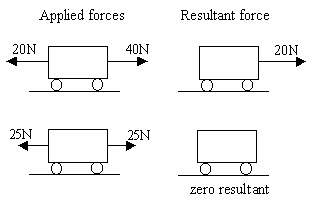
\includegraphics[width=0.5\textwidth]{resultantforce}
  \caption{Examples of net forces. The second truck is in equilibrium, the first experiences an acceleration to the right. \capcite{https://cdn.miniphysics.com/wp-content/uploads/2014/11/forces-in-opposite-direction.jpg}\label{fig:resultant}}
\end{figure}
One of the fundamental ideas of classical physics is that of \textbf{force}. A force is any influence which tends to change the motion of an object
when unopposed. A force is a vector quantity; the \textbf{net force} on an object is the vector sum of all the forces acting on the
object (figure \ref{fig:resultant}).
When the net force is zero, the object is said to be in \textbf{equilibrium}; otherwise the object will accelerate in the direction of
the net force. The unit of force is the newton, N (figure \ref{fig:newton}).
\begin{figure}
  \centering
  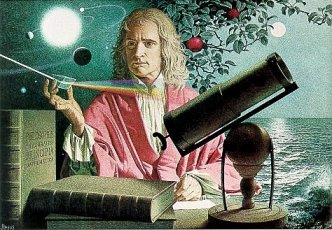
\includegraphics[width=0.7\textwidth]{newton}
  \caption{Sir Isaac Newton. \capcite{http://teachertech.rice.edu/Participants/louviere/Newton/newton5.jpg}\label{fig:newton}}
\end{figure}

\subsection{Examples of Forces}
\begin{itemize}
  \item The normal (support) force is the force which stops things falling through tables (it opposes the force of gravity, and is due to
        the subatomic particles repelling each other).
  \item When an object hangs from a ceiling, or when two objects pull on each other, there is a tension force in the rope connecting them.
  \item Friction forces (like air resistance) oppose movement.
  \item Jet engines produce a thrust force to accelerate aircraft.
  \item Magnets are attracted or repelled through the action of a magnetic force.
  \item Current flows in a wire due to an electric force (in actual fact, the electric and magnetic forces are two viewpoints of the same force...)
  \item The elastic force opposes the stretching of a string.
  \item It is thought that there are four fundamental forces: gravity, the weak nuclear force (governing decay of some subatomic particles),
        the electromagnetic force, and the strong nuclear force (which glues nucleons together).
  \item The `force' from star wars is not a force in the physical sense.
  \item According to general relativity, gravity as a force is only a property of the curvature of space and so is not a `real' force.
  \item The so-called `centrifugal force' is not a force.
\end{itemize}

\subsection{Newton's Laws of Motion}
Sir Isaac Newton described three laws of motion in his \textit{Principia Mathematica} in 1686. The three laws are still a cornerstone
of classical (non-relativistic) mechanics to this day, although they lose accuracy as the velocity of an object tends towards the speed
of light.

\subsubsection{Newton's First Law of Motion} Every object will remain at rest or in uniform motion in a straight line unless compelled
to change its state by the action of an external force.

In other words, an object accelerates if and only if a net force acts on it.

\subsubsection{Newton's Second Law of Motion} The force on an object is simply rate of change of momentum of an object with respect
to time.

We have not yet met the idea of momentum, which is a measure of the total `oomph' an object has. We only need the algebraic consequence
of this law, which is summed up as the following equation:
\begin{equation}
  F_{\text{net}} = ma
\end{equation}

\subsubsection{Newton's Third Law of Motion} For every action (force) in nature there is an equal and opposite reaction.

\textbf{\textcolor{red}{Important idea:}} Forces cause acceleration, and all acceleration is due to a force.

\subsection{Exercises}
\begin{figure}
  \centering
  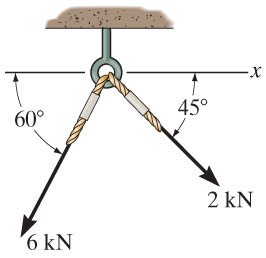
\includegraphics[width=0.3\textwidth]{resultantex}
  \caption{Forces acting on a hook due to a rope. \capcite{http://s3.amazonaws.com/answer-board-image/2ace727f-4377-4440-82e1-17b6311a624b.bmp}\label{fig:resultantex}}
\end{figure}
\begin{enumerate}
  \item A spacecraft moves at a constant speed in a straight line through space. What is the net force on the spacecraft?
  \item A car pulls a caravan. If there is an equal and opposite force opposing the force of the car on
        the caravan, how can the two ever start moving?
  \item Consider figure \ref{fig:resultantex}. What is the net force acting on the eye of the hook?
  \item A tow truck pulls a car of mass \SI{1250}{\kilo\gram} with a force of \SI{1500}{\newton}. If there is
        friction totalling \SI{600}{\newton}, calculate the car's acceleration.
  \item An object of mass \SI{3.0}{\kilo\gram} is held by two strings attached to a roof. The strings are
        each inclined to the vertical at \SI{60}{\degree}. (a) What is the force of gravity on the mass?
        (b) Draw a labelled vector diagram to show that the forces add to give a zero resultant force. (c)
        Calculate the tension $ T $ in each string.
\end{enumerate}

\subsection{Gravity}
Gravity is a force which is exerted by any mass on any other mass. If the two masses $ m $ and $ M $ are a distance $ r $ apart,
then the force between them is given by \textbf{Newton's law of universal gravitation}
\begin{equation}
  F_G = G \frac{mM}{r^2}
\end{equation}
where $ G = \SI{6.674e-11}{\newton\metre\squared\per\kilo\gram\squared} $ is the \textbf{gravitational constant}. This equation
is not examinable at Level 2, but is an important area of study at Level 3. You will, for example, use it to derive the acceleration
due to gravity $ g = \SI{9.81}{\metre\per\second\squared} $.

\subsection{Torque}
\begin{figure}
  \centering
  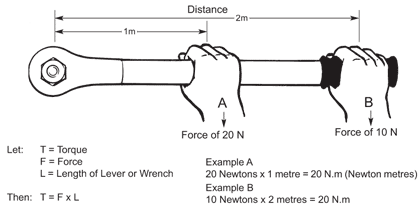
\includegraphics[width=0.8\textwidth]{torque}
  \caption{Torques on a spanner. \capcite{http://www.gedore-torque.com/default/assets//Image/torque-calculation.gif}\label{fig:torque}}
\end{figure}
If we apply a force some distance away from a pivot point, we create a turning effect around the pivot. This turning
effect, which manifests itself as an angular acceleration, is due to \textbf{torque}. Just as force causes linear
acceleration, torque causes angular (rotational) acceleration. If we apply a force $ F $ perpendicular to our level
at a distance $ r $ from the pivot point, we define the torque $ \tau $ (in units of \si{\newton\metre}) to be
\begin{equation}
  \tau = F \times r.
\end{equation}
With this additional concept, we now call an object `in equilibrium' if both the net force and the net torque are zero.

For an example, see figure \ref{fig:torque}. This year, we do not examine rotational physics in detail; an in-depth
discussion of torque is left for Level 3 Physics. However, it is expected that you can do simple calculations involving
torque such as the following exercise:

\paragraph{Exercise.} A painter uses a uniform wooden plank \SI{2.00}{\metre} long and of weight \SI{300}{\newton}.
It is supported at both ends by trestles $ A $ and $ B $. The painter, of weight \SI{800}{\newton}, stands \SI{0.50}{\metre}
from trestle $ A $. Calculate the size of the forces with which trestles $ A $ and $ B $ hold up the plank and the painter.
Note that the weight of the plank acts through its centre of mass. (Hint: write equations for the torque around $ A $
and $ B $ seperately).

\section{Momentum}
Momentum is a quantity describing, in some sense, how much motion an object has. The more momentum an object
has, the more force must be applied to stop it. Momentum is a vector in the same direction as the velocity of
an object, and magnitude given by:
\begin{equation}
  p = mv
\end{equation}

\subsection{Impulse}
When a person wearing ice skates pushes off from a wall, their momentum changes. Obviously then, force causes a change
in momentum --- this can also be seen mathematically, since forces cause acceleration and therefore a change in velocity.

Consider the following reasoning:
\begin{align*}
  F &= ma\\
  &= m \frac{\Delta v}{\Delta t}\\
  &= m \frac{v_f - v_i}{\Delta t}\\
  &= \frac{mv_f - mv_i}{\Delta t}\\
  &= \frac{p_f - p_i}{\Delta t}\\
  \Rightarrow \Delta p &= F \Delta t
\end{align*}

Hence Newton's second law of motion can also be written as
\begin{equation}
  F = \frac{\Delta p}{\Delta t} = \od{p}{t}.
\end{equation}

A change in momentum is also called an \textbf{impulse}; the two have equivalent units, but it is standard to write impulse in
terms of \si{\newton\second} and momentum in terms of \si{\kilo\gram\meter\per\second}. The symbol for impulse is $ J $.

\begin{equation}
  J = F \Delta t = \rint F \dif{t}
\end{equation}

\paragraph{Exercise.} A lump of blu-tack of mass \SI{100}{\gram} falls, hits the ground at \SI{4.0}{\metre\per\second}, and stops. Calculate
the magnitude of the ball's change in momentum.

\subsection{Conservation of Momentum}
\begin{figure}
  \centering
  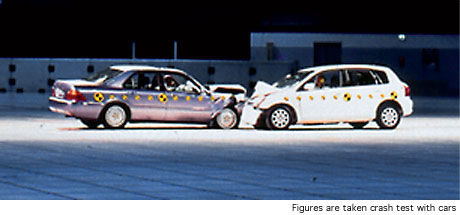
\includegraphics[width=0.4\textwidth]{carcrash}
  \caption{An inelastic collision. \capcite{http://world.honda.com/factbook/auto/motorshow/200110/img/12_p02.jpg}\label{fig:baddriver}}
\end{figure}
Momentum is most useful when modelling collisions, because the total momentum of a `nice' system is always conserved --- i.e. a system which is
not made up of smaller things that can move around on their own. This is called the \textbf{law of conservation of momentum}.

Of course, no `real' collision is really momentum-conserving: the problem is that all things at a macroscopic level are made up of smaller things,
so some of the momentum is transferred into moving those smaller things! The existence of smaller particles inside the proton, for example, was
discovered by firing electrons at the nucleus and comparing the momentum of the system beforehand to the momentum after the collision, and noticing
that something inside the proton must have jiggled.

A collision in which kinetic energy as well as momentum is conserved is called an \textbf{elastic collision}. Remember that it is \emph{energy in general} that
is conserved, not kinetic energy --- energy is allowed to change forms. \emph{Most collisions are inelastic}.

The car crash shown in figure \ref{fig:baddriver} is inelastic, because energy gets transformed into heat and sound as the metal
crumples. Obviously the mass of the cars doesn't change (unless the collision is either exceptionally violent, or the cars were
travelling close to the speed of light), but both come to a halt --- so the momentum cannot have been conserved either!

It is also important to remember that \emph{momentum is a vector quantity}, and so the direction of collision can be important!

\paragraph{Example of a conservation problem (2016 paper, merit).} A red car, moving with the speed of \SI{1.5}{\metre\per\second},
collides with a stationary blue car. The mass of the red car is \SI{0.050}{\kilo\gram}, and the mass of the blue car is
\SI{0.040}{\kilo\gram}. If the velocity of the blue car after the collision is \SI{1.2}{\metre\per\second}, calculate the
velocity of the car after the collision.

\paragraph{Solution.} The initial momentum is $ v_{\text{red}} m_{\text{red}} = 1.5 \cdot 0.05 = \SI{0.075}{\kilo\gram\metre\per\second} $.
This must equal the sum of the final momentums of both cars. The final momentum of the blue car is $ p_{\text{blue}} = 1.2 \cdot 0.04 =
\SI{0.048}{\kilo\gram\metre\per\second} $, hence the final momentum of the red car is \SI{0.027}{\kilo\gram\metre\per\second} and its
final velocity is \SI{0.54}{\metre\per\second}.

\begin{center}
\begin{tcolorbox}[width=0.8\textwidth,colback={red},title={\textbf{Go and watch...}},colbacktitle=yellow,coltitle=blue]
  \textcolor{white}{\url{https://www.youtube.com/watch?v=2UHS883_P60}}
\end{tcolorbox}
\end{center}

\begin{figure}
  \centering
  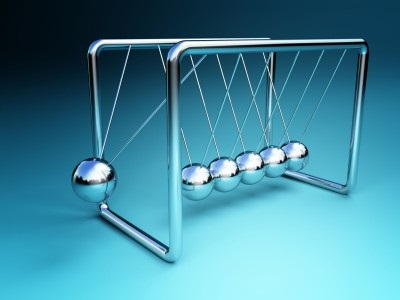
\includegraphics[width=0.5\textwidth]{newtoncradle}
  \caption{Newton's Cradle, a popular desktop toy. \capcite{http://images.tutorvista.com/cms/images/95/conservation-of-momentum-experiment1.jpg}\label{fig:babynewton}}
\end{figure}

\paragraph{Exercise.} Explain now a Newton's Cradle works (figure \ref{fig:babynewton}).

\paragraph{Exercise.} A small child of mass \SI{25}{\kilo\gram} runs into a beanbag with a speed of \SI{0.5}{\metre\per\second} and is brought to a
halt. The collision occurs over a time period of \SI{2}{\second}. (a) What was the change of momentum of the child? (b) What was the total force
exerted by the beanbag on the child? (c) What was the total force exerted by the child on the beanbag? (d) The final momentum of the child-beanbag
system is zero, since neither is moving. Why does this not violate conservation of momentum?

\begin{figure}
  \centering
  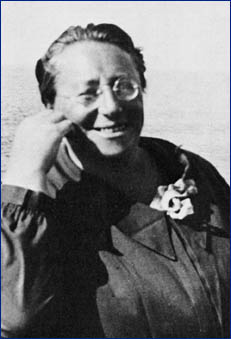
\includegraphics[width=0.4\textwidth]{noether}
  \caption{Emmy Noether. \capcite{http://www.amt.edu.au/images/root-imgs/biognoether.jpg}\label{fig:noether}}
\end{figure}
One of the people who contributed most to the modern understanding of conservation laws was Emmy Noether (figure \ref{fig:noether}); Noether's
theorem states that every conservation law is associated with a symmetry in the mathematical laws of physics (and conversely, every symmetry
in the laws of physics is associeted with a conservation law). She is now recognised as one of the most influential people in theoretical physics
and abstract algebra (she also worked on revolutionary ideas in ring theory) at the time.

\section{Energy}
\begin{figure}
  \centering
  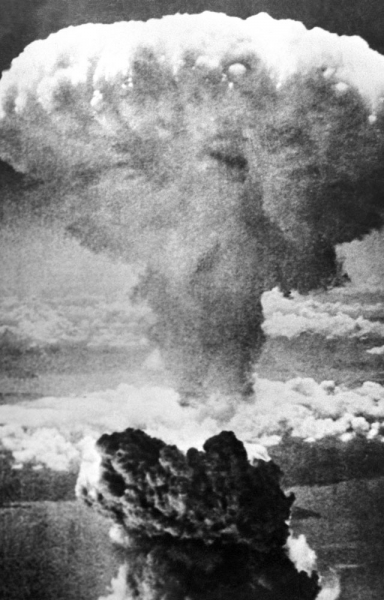
\includegraphics[width=0.5\textwidth]{energy}
  \caption{When energy is released, the results can be incredibly powerful. The atomic bomb dropped by the USA on Nagasaki, Japan in 1945 released \SI{84}{\tera\joule} of energy, but its power is probably better measured by the death toll which some estimates put over 100,000 people. \capcite{http://cdn3-europe1.new2.ladmedia.fr/var/europe1/storage/images/media/images/nagasaki/21361791-1-fre-FR/Nagasaki_reference.jpg}\label{fig:atom}}
\end{figure}
Another quantity which is always conserved in a closed system is \textbf{energy}. Simply put, energy is the ability
of an object to do something interesting. The more energy an object has, the bigger the `stuff' it can do. Energy is
used to do stuff when it is transformed from one form (like kinetic energy) into another (like heat energy). This
process is called doing \textbf{work}, and in Level 1 we saw that the work done $ W $ is related to how much force is felt ---
the work done is equal to the force $ F $ multiplied by the distance the object travels \textbf{in the direction of the force}.
\begin{equation}
  \Delta E = W = Fd
\end{equation}
In other words, one joule of work is done (one joule of energy is transformed from one form into another) when an object
is moved using a force of one newton over a distance of one metre.

\textbf{By itself, energy is just a number. It's only important when it gets transformed from one form to another.} Energy is
a measure of the possibility of doing work, and work is a measure of how much stuff something has done.

The rate at which energy is transferred (the rate at which work is done) is called \textbf{power}; as usual for calculating
rates, we can write
\begin{equation}
  P = \frac{W}{\Delta t} = \od{E}{t}. \label{eqn:power}
\end{equation}
The unit for power is the watt (W), named for the Scottish inventor James Watt (figure \ref{fig:watt}) who worked
on steam engines during the industrial revolution.

\begin{figure}
  \centering
  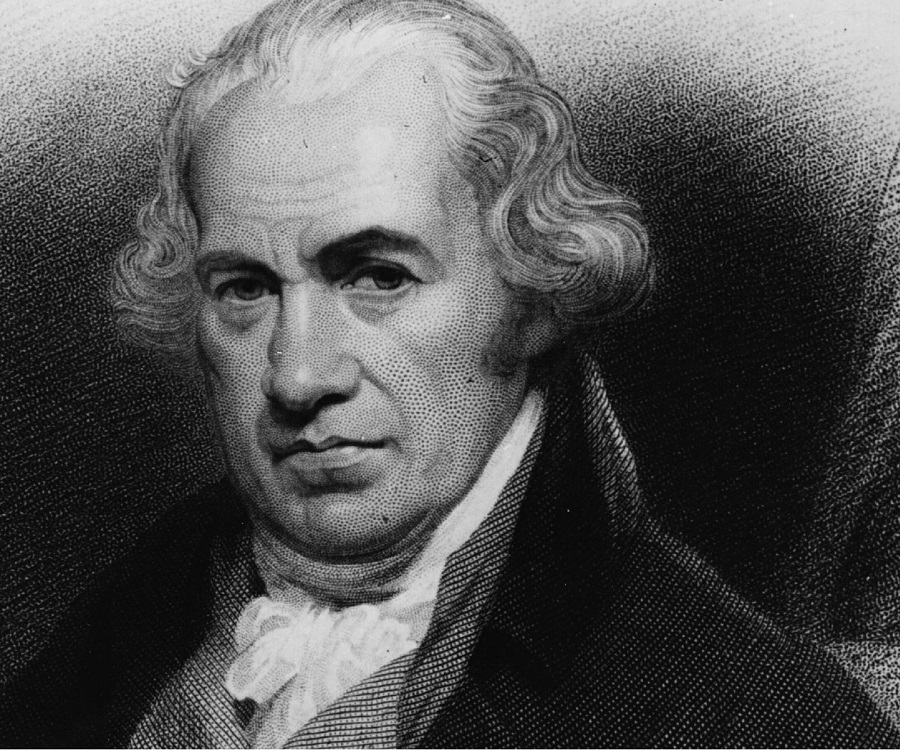
\includegraphics[width=0.4\textwidth]{watt}
  \caption{James Watt. \capcite{https://www.thefamouspeople.com/profiles/images/james-watt-3.jpg}\label{fig:watt}}
\end{figure}

The \textbf{law of conservation of energy} states that \textit{energy can never be created or destroyed, only transferred
from one form to another}. It has actually been shown that energy can be transformed into mass and vice-versa, so in reality
it is \textit{mass-energy} (the sum of the energy of the object and the energy-equivalent of the mass of the object) that is
conserved. However, if there is no conversion between mass and energy taking place (such as when we aren't dealing with nuclear
reactions or really small or fast things) the simple version works perfectly well. The simple law of conservation of energy will
hold in all of the work you do at Level 2 (outside, maybe, of the modern physics standard).

\subsection{Gravitational Potential Energy}
Suppose an object of mass $ m $ is lifted aginst gravity at a constant speed to a height $ h $. Then the force needed to do
the lifting is the weight of the object, $ W = mg $, and the work done is
\begin{equation}
  \Delta E_g = mgh
\end{equation}
where $ g = \SI{9.81}{\metre\per\second\squared} $ is the acceleration due to gravity. The energy of the thing doing the lifting
(perhaps chemical energy in the fuel tank of a forklift) is converted into \textbf{gravitational potential energy}.

\paragraph{Exercise.} How does gravity act over a distance? It works in a vacuum too, but how? (Think fields.)

\subsection{Kinetic Energy}
Objects in motion have some energy due to that motion (if you stick your hand in front of a moving bus, it will probably
hurt as the bus does work on your hand --- and in order to do work, it must have energy). We can calculate the \textbf{kinetic energy}
of a moving object to be
\begin{equation}
  E_k = \frac{1}{2} mv^2 = \frac{p^2}{2m}.
\end{equation}

\paragraph{Exercise.} A car is moving at a constant speed with kinetic energy $ E_k $ when the engine is cut off. The car coasts to a halt,
and so its final kinetic energy is zero. Why does this loss of kinetic energy not violate the law of conservation of energy?

\paragraph{Exercise.} A bullet of mass \SI{30}{\gram} is fired horizontally with a speed of \SI{400}{\metre\per\second} into
a sandbag of mass \SI{10}{\kilo\gram} that is free to swing with negligible friction. What is the maximum vertical height $ h $
that the sandbag rises as it recoils with the bullet lodged inside?

\subsection{Elastic Potential Energy}
\begin{figure}
  \centering
  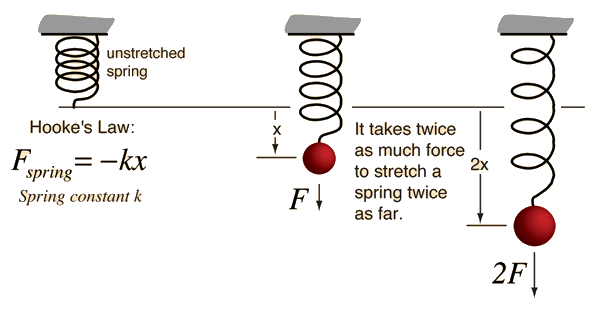
\includegraphics[width=0.9\textwidth]{hooke}
  \caption{Springs can be modelled using Hooke's Law. \capcite{http://hyperphysics.phy-astr.gsu.edu/hbase/imgmec/hook.gif}\label{fig:hookeslaw}}
\end{figure}
\begin{figure}
  \centering
  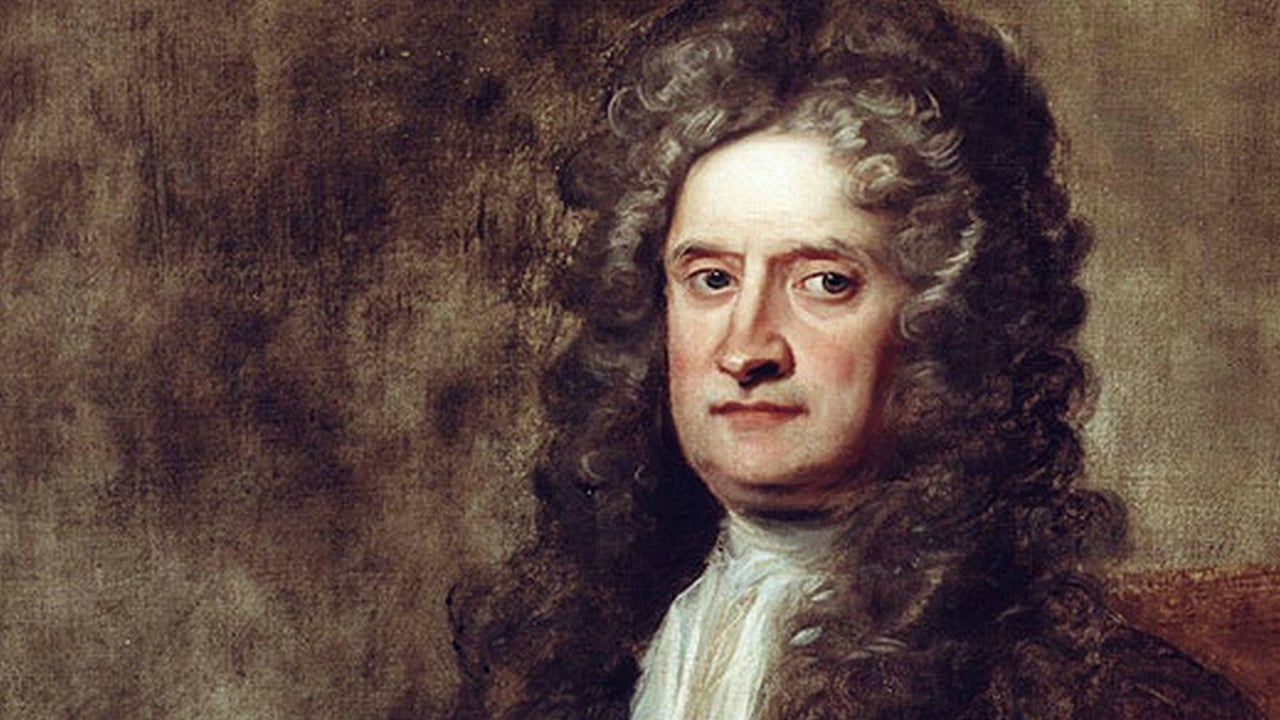
\includegraphics[width=0.5\textwidth]{hookeman}
  \caption{Robert Hooke. \capcite{https://i.vimeocdn.com/video/496483451_1280x720.jpg}\label{fig:hooke}}
\end{figure}
When compressing or stretching a string or a rubber band, work is done. Some of the energy is transformed into
heat energy, but other energy must be stored as \textbf{elastic potential energy} in the spring (since if you let go,
it rebounds to almost its original position). It can be found experimentally that for small compressions or stretches,
the total force required is directly proportional to the displacement from the zero point. We therefore have \textbf{Hooke's Law},
\begin{equation}
  F = -kx
\end{equation}
where $ k $ is a constant that depends on the particular spring. A graphical depiction of Hooke's Law can be seen in figure \ref{fig:hookeslaw}.

Robert Hooke (figure \ref{fig:hooke}), the English scientist after whom the law is named, is more famous for inventing the microscope and coining the term `cell'
for the small self-contained parts of living organisms.

A formula for elastic potential energy can be found by integrating under the curve of force over distance for Hooke's Law.
\begin{equation}
  \Delta U_{\text{elastic}} = \frac{1}{2} kx^2
\end{equation}

\begin{center}
\begin{tcolorbox}[width=0.8\textwidth,colback={red},title={\textbf{Go and watch...}},colbacktitle=yellow,coltitle=blue]
  \textcolor{white}{\url{https://www.youtube.com/watch?v=G_22yf_gJyg}}
\end{tcolorbox}
\end{center}

\paragraph{Exercise.} A bungy jumper of mass \SI{75}{\kilo\gram} jumps off a bridge over a river. The spring constant
of the rope is such that the jumper's head just touches the water at maximum stretch (\SI{30}{\metre}). If the natural
length of the rope is \SI{10}{\metre}, calculate the spring constant of the rope. You may assume that no energy is lost
to friction.

\subsection{A Note on Notation}
Work, energy, and potential energy are all basically the same thing. I tend to use $ E $, $ W $, and $ \Delta U $ respectively
for them; the main confusion comes in the final chapter, where we use $ E $ to denote the electric field vector at a point.

\section{Projectile Motion}
\begin{figure}
  \centering
  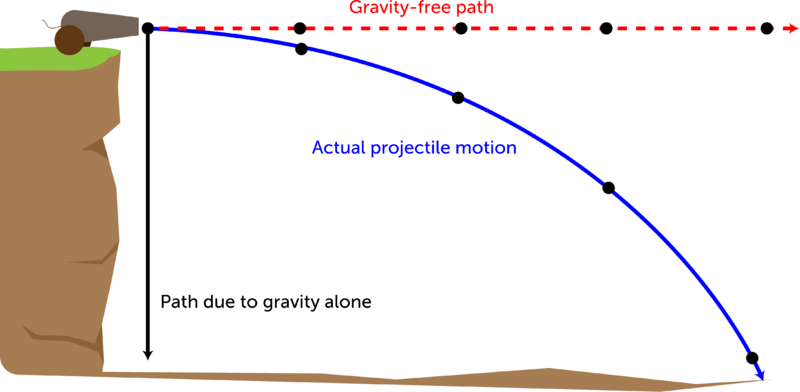
\includegraphics[width=0.9\textwidth]{projectile}
  \caption{Projectiles are only acted upon by gravity. \capcite{http://cimg2.ck12.org/datastreams/f-d\%3Abb024be6673110b31e78b46819e792adaed8dc661e082a61f0a6d64e\%2BIMAGE\%2BIMAGE.1}\label{fig:projectile}}
\end{figure}
\begin{figure}
  \centering
  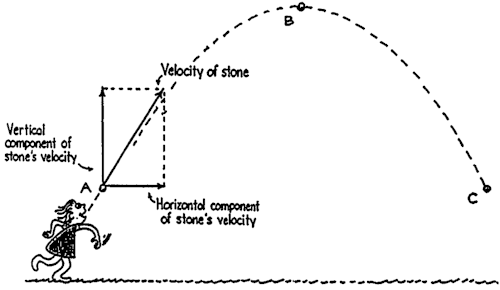
\includegraphics[width=0.6\textwidth]{components}
  \caption{Projectile motion can be modelled by splitting up the horizontal and vertical components of motion. \capcite{http://dev.physicslab.org/img/06743d2f-de75-41fd-8b87-7130f9112bbb.gif}\label{fig:components}}
\end{figure}
Gravity is an important force in everyday life, and its effects in some cases can be easy to undertand. One such case
is a type of motion called \textbf{projectile motion}. A projectile is an object moving through the air such that the
only force acting on it is gravity --- for example, a cannon ball (if we neglect air resistance).

Our simplified model of projectiles has several important consequences (figure \ref{fig:projectile}):
\begin{itemize}
  \item A particle undergoing projectile motion accelerates constantly downwards (the acceleration due to gravity
        is $ g = \SI{9.81}{\metre\per\second\squared} $, and is essentially constant everywhere around the planet).
  \item Since there is no force acting in the horizontal direction, the particle's horizontal velocity remains constant.
\end{itemize}
Particles undergoing projectile motion follow a parabolic path.

In order to calculate (for example) the range of a particle undergoing projectile motion, we must therefore split
the velocity into components (figure \ref{fig:components}). If the particle has an initial velocity $ v $ at an angle $ \theta $
with the horizontal, then the two components of velocity will be $ v_x = v \cos \theta $ and $ v_y = v \sin \theta $. We can then
find the time taken for the particle to rise up to its peak using the kinematic equations --- we know the initial vertical
velocity is $ v_y $, the final velocity is 0, and the acceleration is $ -g $, so it is a simple matter to find the time $ t $ taken.
Then we know that the time taken in total for the particle to rise up and fall back down to earth is $ 2t $, and therefore
the range is $ v_x \cdot 2t $.

\begin{center}
\begin{tcolorbox}[width=0.8\textwidth,colback={red},title={\textbf{Go and watch...}},colbacktitle=yellow,coltitle=blue]
  \textcolor{white}{\url{https://www.youtube.com/watch?v=97VV_lrwn9Y}}
\end{tcolorbox}
\end{center}

\subsection{Exercises}
\begin{enumerate}
  \item `In real life, no object is ever a true projectile.' Discuss.
  \item How high does a golfball rise if it is hit with an initial speed of \SI{40}{\metre\per\second} at an angle
        of \SI{40}{\degree} to the ground?
  \item A javelin is thrown at a speed of \SI{20}{\metre\per\second} at an angle of \SI{30}{\degree} to the ground. By modelling
        the javelin as a projectile, compute the distance from the throwing point at which the javelin hits the ground.
  \item A small ball is fired directly upwards from a moving vehicle. Describe the motion of the vehicle so that the ball falls
        back into it, and describe the motion of the ball.
\end{enumerate}

\section{Circular Motion}
\begin{figure}
  \centering
  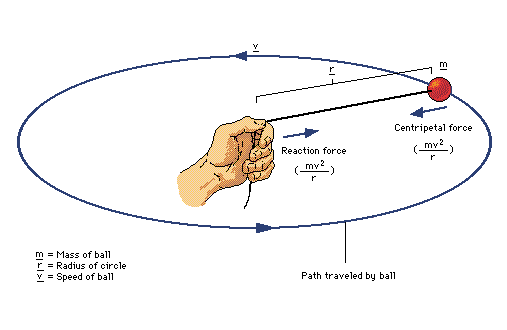
\includegraphics[width=0.9\textwidth]{centripetal}
  \caption{A force which causes circular motion is called a centripetal force. \capcite{https://i.pinimg.com/originals/74/d2/28/74d228e85a6a3f4fb700bcafa677539d.gif}\label{fig:centripetal}}
\end{figure}
This year, we also consider a limited form of motion in a circle --- when the object is moving at a constant speed. Suppose
a particle moves in a circle of radius $ r $ with constant velocity (around the edge of the circle) $ v $. We call the time
taken for one full rotation the \textbf{period} $ T $ of the motion; the frequency $ f $ is the number of times per second
that the particle rotates and (as in wave motion) is given by $ f = \frac{1}{t} $. Since the circumference of a circle is
given by $ C = 2\pi r $, we have the following formula (where $ \omega = 2\pi f $ is called the \textbf{angular frequency}):
\begin{equation}
  v_{\text{rot}} = \frac{2\pi r}{T} = 2\pi f r = \omega r
\end{equation}

Obviously the particle's direction is changing and so its velocity is changing (even though the speed is constant). This means
that there must be an acceleration acting on the particle that points directly into the circle at right angles to the particle's
motion (the angle must be \SI{90}{\degree}, otherwise the speed of the particle would change as well as the direction). By
our work previously, we know that this acceleration must be due to some kind of force. We call this force a \textbf{centripetal
force} (figure \ref{fig:centripetal}).

\paragraph{Exercise.} What causes the centripetal force causing the Moon to orbit the Earth?

\begin{center}
\begin{tcolorbox}[width=0.8\textwidth,colback={red},title={\textbf{Go and watch...}},colbacktitle=yellow,coltitle=blue]
  \textcolor{white}{\url{https://www.youtube.com/watch?v=KvCezk9DJfk}}
\end{tcolorbox}
\end{center}

You may have heard of centrifugal force, but it is in fact a fictional force --- if you feel pushed outwards in a turning car,
what you're actually feeling is your body's resistance to acceleration rather than any physical force. If you look into
the car from the outside, no force is observed and therefore the force cannot exist (a force is always observable in any
reference frame, and if a `force' is observable from one place but not another then it cannot be a real force).

\begin{center}
\begin{tcolorbox}[width=0.8\textwidth,colback={red},title={\textbf{Go and watch...}},colbacktitle=yellow,coltitle=blue]
  \textcolor{white}{\url{https://www.youtube.com/watch?v=zHpAifN_2Sw}}
\end{tcolorbox}
\end{center}

We can calculate the centripetal acceleration to be
\begin{equation}
  a = \frac{v^2}{r}
\end{equation}
and therefore the centripetal force acting on an object of mass $ m $ undergoing circular motion is
\begin{equation}
  F = ma = \frac{mv^2}{r}.
\end{equation}

\paragraph{Exercise.} A \SI{7.0}{\kilo\gram} steel ball is swung horizontally in a \SI{2}{\metre}-radius circle at
a constant speed of \SI{10}{\metre\per\second}. Find the net force on the ball.

\paragraph{Exercise.} A very tall man whirls a \SI{0.50}{\kilo\gram} stone above his head at the end of
a \SI{2.0}{\metre} length of fishing line. The line has a breaking strain of \SI{25}{\newton}.
He increases the speed of the stone until the line breaks; what is the speed of the stone
at this time?

\paragraph{Exercise.} Show that an equivalent formula for centripetal force is
\begin{displaymath}
  F = \frac{4\pi^2 mr}{T^2}
\end{displaymath}

\chapter{91173: Demonstrate Understanding of Electricity and Magnetism}
\begin{center}
  \textcolor{red}{Ensure that you care comfortable with vectors before attempting this chapter! They are even more important
  here than in mechanics.}
\end{center}

\section{On Electromagnetism}
Electromagnetism is probably one of the NCEA standards most removed from everyday life --- we see the effects
of electricity and magnets everywhere, but unlike mechanics or waves we cannot directly experience the world
which we will start to describe this year. Let us take a trip back in time...

Suppose we rub some plastic rods with wool and try to bring them together. It requires a bit of force to do so,
which is odd since we see no change in either rod; nor can we understand what may have rubbed off the wool onto
the rod (or vice versa)! We also observe that a glass rod rubbed with silk attracts slightly the plastic rod,
and that neither rod exhibits this behaviour before it is rubbed. We decide to call objects with this strange new
property \textbf{charged}, and objects without it (like the unrubbed rods) \textbf{neutral}. We know that there
seem to be two varieties of this charge, and that it seems to be able to be transferred from object to object.

Further experiment shows that in some substances, like metal, if one end is rubbed then the other end instantly
seems to become charged as well. The plastic and glass rods do not exhibit this property --- if we rub one end,
only that end becomes charged. We call substances like the metal \textbf{conductors}, and substances that do not
conduct this charge \textbf{insulators}.

Fast forward now to the modern day. We now have a much better understanding of this world of invisible properties
and strange forces; we call the two types of charge \textbf{positive} (glass rod) and \textbf{negative} (plastic rod),
and we have harnessed the power of this \textbf{electric charge} to power our homes and our industry.

We know now that everyday matter is made up of atoms, which contain tiny positive particles (protons) and even tinier
negative particles (electrons). An object which has a net negative charge has more electrons than protons, and an
object with a net positive charge has more protons. A neutral (uncharged) object has equal numbers of protons and
electrons. Note that these subatomic particles are still governed by Newton's laws: an object cannot become charged
instantaneously, a charged particle must first jump to it. When we rubbed a plastic rod with wool, at a subatomic
level the friction between the two substances broke the bonds holding electrons within the atoms of the wool and
the electrons jumped onto the rod, creating a net charge on each.

\begin{figure}
  \centering
  \includegraphics[width=0.4\textwidth]{coulomb}
  \caption{Charles-Augustin de Coulomb. \capcite{https://i.pinimg.com/736x/c1/d3/ab/c1d3abe6a6b800a8bfad883ccff23b5e--coulomb-scientists.jpg}\label{fig:coulomb}}
\end{figure}
Electric charge is measured in coulombs (C). The unit is named after Charles-Augustin de Coulomb (figure \ref{fig:coulomb}), a French physicist
who studied the laws governing the electric field of a point charge. We usually use the letter $ Q $ to denote charge, since before electrons
were discovered, scientists talked about the \textbf{Q}uantity of electricity in a region. The charge on a proton is \SI{1.6e-19}{\coulomb},
and the charge on an electron is equal and oposite to this.

\section{Electric Fields}
\begin{figure}
  \centering
  \includegraphics[width=0.6\textwidth]{fieldlines}
  \caption{The electric field surrounding two protons. \capcite{http://www.physicsclassroom.com/Class/estatics/u8l4c7.gif}\label{fig:fieldlines}}
\end{figure}
An \textbf{electric field} is a region of space in which charged objects feel an \textbf{electrostatic force}; the
space could be empty, or it could be filled with matter (for example, a wire). Every charged object creates a magnetic
field around itself, and every charged object is affected by a magnetic field.

At any given point in space, the \textbf{field value} is a \textit{vector} pointing in the direction that a positive
charge would feel a force. Fields radiate out from positive charges, and radiate in towards negative charges. We
represent electric fields graphically using field diagrams, like figure \ref{fig:fieldlines}. Field lines represent the direction of
the electric field at each point; the closer together the lines, the stronger the field.

Field lines radiate out at right angles from charges, cannot cross each other (why?), and always begin and end at charges.

We have described the direction of the field at every point now; the magnitude is simply the force felt by a test particle
of unit charge at that point. Mathematically, we have
\begin{equation}
  E = \frac{F}{q}
\end{equation}
where $ F $ is the force felt by a particle of charge $ q $ at the given point. The unit for field strength is \si{\newton\per\coulomb}.

If a point charge is placed in a field generated by another point particle, the force it feels is inversely proportional to the distance
it is from the originating particle (in fact, the law for force strength in this case is known as \textit{Coulomb's Law} and is an inverse
square law, like gravity).

Note that there is \textit{only one `electric field'}. Charged particles change the value of this field by being in space, but even when
there is no charge around the field exists --- it just has a value of zero. When two charged particles are close together, the electric
fields that they generate add together (just like the superposition of waves). The value of \textbf{the} electric field at a point is just
the sum of the individual contributions to the fields made by charged objects.

\textbf{\textit{The electric field is just made up of a vector at every point in space, that contains information about the strength and
direction of the field at that point.}}

Remember, \textit{field lines are a convenient fiction} --- they help us understand what's going on, but there's still field where there are
no lines! They just help us to show in a diagram what the field is generally doing within some area of space at some instant in time.

\begin{center}
\begin{tcolorbox}[width=0.8\textwidth,colback={red},title={\textbf{Go and watch...}},colbacktitle=yellow,coltitle=blue]
  \textcolor{white}{\url{https://www.youtube.com/watch?v=nxi8hGeicCM}}
\end{tcolorbox}
\end{center}

It is possible to calculate the magnitude of the electric field due to some point charge $ q $ at an observation location a distance $ r $
from the point charge using \textbf{Coulomb's law}:
\begin{equation}
  E = \frac{1}{4\pi \epsilon_0} \frac{q}{r^2}
\end{equation}
where $ \epsilon_0 = \SI{8.85e-12}{\coulomb\squared\per\newton\metre\squared} $ is called the \textbf{permittivity of free space}.
Like gravity, Coulomb's law is an inverse-square law. It is not examinable at Level 2.

\section{Electric Potential Energy and Voltage}
Electric fields are similar to gravitational fields in several ways. For example, both have some notion of potential energy associated
with them. Consider a particle of mass $ q $ in a uniform electric field of strength $ E $. If we move this particle against the field
for a distance $ \Delta x $, we do work on the particle of magnitude $ W = F \Delta x $.  But we know that $ F = Eq $, and so the work
done is $ W = Eq \Delta x $. Hence the change in potential energy of the particle is
\begin{equation}
  \Delta U_{\text{electric}} = E q \Delta x.
\end{equation}
The similarity to the equation for $ E_g $ is apparent: $ \Delta x $ corresponds to height, $ q $ to mass, and $ E $ to the acceleration
due to gravity.

The change in energy per unit charge over a given distance is called the \textbf{electric potential difference} or \textbf{voltage difference}
between those points. The units of voltage are volts (V), and by definition the voltage difference over a distance $ \Delta x $ is
\begin{equation}
  \Delta V = E \Delta x
\end{equation}
This allows us to define another unit for electric field strength, \si{\volt\per\metre}.

\textcolor{red}{\textbf{Electric potential} and \textbf{electric potential energy} are two entirely different concepts: the first is voltage,
a property of a point in space; the second is the property of a charged particle in that space.}

\begin{figure}
  \centering
  \includegraphics[width=0.6\textwidth]{ground}
  \caption{The grounding point of a home. \capcite{https://upload.wikimedia.org/wikipedia/commons/thumb/7/7d/HomeEarthRodAustralia1.jpg/250px-HomeEarthRodAustralia1.jpg}\label{fig:ground}}
\end{figure}

As with gravitational potential energy, we must pick some location to act as `zero' for electric potential. We generally use the earth
as our zero reference point, and this is called the \textbf{ground}. In a domestic setting, it is usual to see metal stakes driven into
the ground (as in figure \ref{fig:ground}) to set the reference voltage. They also have a second job: in the event of a short circuit,
all the current in the house is dumped straight into the earth in order to prevent electrical accidents.

Charge moves from a point with a higher voltage to a point with a lower voltage. A battery produces a voltage difference across its terminals
in order to push charge around the circuit. If we look at a positive charge, which moves in the direction of field lines, we see that as we move
down a field line the voltage will decrease.

Noting that we have
\begin{equation}
  E = \frac{\Delta V}{\Delta x} = \od{V}{x},
\end{equation}
we have another intuitive viewpoint of a field: the rate of change of potential difference. As we move from points of low voltage
to points of high voltage, we move up the field; so the electric field points in the opposite direction to that in which the potential
increases. In fact, if we have some reference (a `zero point', like the ground) then voltage forms a field --- just one made up of
numbers rather than vectors. The reason we talk about electric fields but not voltage fields is that the former encode much more information
and we can work out the voltages with the electric field anyway.

\begin{center}
\begin{tcolorbox}[width=0.8\textwidth,colback={red},title={\textbf{Go and watch...}},colbacktitle=yellow,coltitle=blue]
  \textcolor{white}{\url{https://www.youtube.com/watch?v=f0AQpjh3G9o}}
\end{tcolorbox}
\end{center}

\subsection{Exercises}
The mass of an electron is \SI{9.11e-31}{\kilo\gram}, and the charge on an electron is \SI{-1.60e-19}{\coulomb}.
\begin{enumerate}
  \item Show that the units \si{\newton\per\coulomb} and \si{\volt\per\metre} are equivalent.
  \item Two parallel metal plates \SI{2.0}{\milli\metre} apart have a potential difference of \SI{48}{\volt} applied
        to them. A speck of dust is placed midway between the plates; the speck has collected $ 10^{12} $ extra electrons
        on itself. Find the electric field strength between the plates, and the magnitude and direction of the electric
        force on the speck of dust.
  \item Which of the following statements is \textbf{not} true?
    \begin{enumerate}
      \item Electric potential (voltage) exists everywhere, whether or not a charged particle is there to experience it.
      \item The electric potential energy is created by the interaction of a charged particle with the source charges.
      \item A battery marked \SI{1.5}{\volt} has an electric potential energy of \SI{1.5}{\volt}.
      \item A positive charge slows down as it moves into a region of higher electric potential.
    \end{enumerate}
  \item There are three different configurations of charges: one electron and one proton at a distance of $ r $;
        one electron and one proton at a distance of $ 2r $; and two protons at a distance of $ r $. In which case
        will it require the most work to seperate the charges to infinity? (Hint: you should not need to perform
        any calculations.)
  \item What is the speed of an electron that has been accelerated from rest through a potential difference of \SI{1000}{\volt}?
        (Hint: find the electrical potential energy lost and then use conservation of energy. Don't worry about your potential energy
        being negative, it just means that the P.E. is less than our totally arbitrary zero point.)
\end{enumerate}

\section{Direct Current}
\begin{figure}
  \centering
  \includegraphics[width=0.6\textwidth]{current1}
  \caption{Electrons flowing in a conductor. \capcite{https://www.sciencebuddies.org/Files/6631/7/wire-conventional-current.png}\label{fig:current1}}
\end{figure}
\begin{figure}
  \centering
  \includegraphics[width=0.6\textwidth]{current2}
  \caption{Conventional current versus electron flow. \capcite{http://www.talkingelectronics.com/projects/Diode\%20-\%20How\%20A\%20Diode\%20Works/images/CurrentFlow-2.gif}\label{fig:current2}}
\end{figure}
\begin{figure}
  \centering
  \includegraphics[width=0.6\textwidth]{current3}
  \caption{Hovertext: Sure, we could stop dictators and pandemics, but we could also make the signs on every damn diagram make sense. \capcite{https://xkcd.com/567/}\label{fig:current3}}
\end{figure}
\begin{figure}
  \centering
  \includegraphics[width=0.4\textwidth]{ampere}
  \caption{Andr\'e-Marie Ampere, the namesake of the unit of current. \capcite{http://www.nndb.com/people/574/000097283/ampere-1.jpg}\label{fig:ampere}}
\end{figure}
We now move from considering fields in space and point charges, to discussing the organised movement
of charges in a conductor. By definition, this flow is called \textbf{current}; we define the current vector
at a point to be:
\begin{equation}
  I = \frac{\Delta Q}{\Delta t} = \od{Q}{t}
\end{equation}
The units of current are amperes (A), named after Andr\'e-Marie Ampere (figure \ref{fig:ampere}), a French physicist and founder
of electromagnetism as a modern field of study. The symbol $ I $ comes from the French \textit{intensit\'e de courant}.

If you've done the Level 2 Chemistry standard `91164: Demonstrate understanding of bonding, structure, properties and energy changes',
then you'll be aware that a metal is made of a lattice of positive charges (atomic nuclei) surrounded by a sea of delocalised electrons;
it is these electrons that flow to form a current when an electric field (or equivalently a potential difference) is applied across the
metal. Note that the `real' flow speed of the electrons is really slow --- in a copper wire, the drift speed of electrons is around
\SI{23}{\micro\metre\per\second}.

\paragraph{Exercise.} If electrons move so slowly, why does a light turn on almost instantaneously when a switch is flipped? (Hint: think
about squeezing a tube of toothpaste.)

\subsection{Direction of Current}
When drawing diagrams, there is a difference between \textbf{electron current} and \textbf{conventional current}.
The former is the flow of electrons in a wire, and the latter is in the opposite direction. Recall that electric
field vectors are defined to point in the direction of movement of a positive charge; this means that the electric
field causing the current flow points in the direction of the conventional current rather than the direction of the
movement of electrons (see figures \ref{fig:current1} and \ref{fig:current2}).

The reason that everything is based off positive charges rather than negative charges (the ones that actually move)
is purely historical (figure \ref{fig:current3}). In some conductors, like ionic solutions, both positive and negative
charges flow; in this case, conventional current still follows the direction of flow of the positive charges.

\begin{center}
\begin{tcolorbox}[width=0.8\textwidth,colback={red},title={\textbf{Go and watch...}},colbacktitle=yellow,coltitle=blue]
  \textcolor{white}{\url{https://www.youtube.com/watch?v=fBNLzgr9T6w}}
\end{tcolorbox}
\end{center}

\begin{center}
\begin{tcolorbox}[width=0.8\textwidth,colback={red},title={\textbf{Go and watch...}},colbacktitle=yellow,coltitle=blue]
  \textcolor{white}{\url{https://www.youtube.com/watch?v=-Rb9guSEeVE}}
\end{tcolorbox}
\end{center}

\subsection{Circuit Diagrams}
\begin{figure}
  \centering
  \includegraphics[width=0.4\textwidth]{schematic}
  \caption{A simple electric circuit, consisting of a battery (cell), a switch, and a lamp. \capcite{http://www.thunderboltkids.co.za/Grade6/03-energy-and-change/images/gd-0033.png}\label{fig:schematic}}
\end{figure}
\begin{figure}
  \centering
  \includegraphics[width=0.6\textwidth]{schematic2}
  \caption{A more complicated circuit. \capcite{https://xkcd.com/730/}\label{fig:schematic2}}
\end{figure}
\begin{figure}
  \centering
  \includegraphics[width=0.6\textwidth]{circuitelements}
  \caption{Various components which can be used in circuit diagrams. \capcite{https://i.pinimg.com/originals/cb/26/ca/cb26ca8e687eeb42ec39f03b2944a98d.png}\label{fig:circuitelements}}
\end{figure}
A \textbf{circuit} is a path around which electrons can flow. The different parts of the circuit, like batteries and
lamps, are called \textbf{components}. We usually draw electric circuits in the form of a schematic, or a \textbf{circuit
diagram}, like figure \ref{fig:schematic}. A table of different symbols for components is given in figure \ref{fig:circuitelements}; as
we diiscuss different components this year, we will reintroduce several of these symbols one-by-one.

\subsection{Batteries}
\begin{figure}
  \centering
  \includegraphics[width=0.4\textwidth]{battery}
  \caption{A typical battery. Other brands are available. \capcite{http://www.thewarehouse.co.nz/on/demandware.static/-/Sites-twl-master-catalog/default/dw84dabfe4/30/67/R458734_00.jpg}\label{fig:battery}}
\end{figure}
A \textbf{battery} (or \textbf{cell}) is a component that creates a potential difference across its two ends. A \SI{9}{\volt}
battery like that in figure \ref{fig:battery} creates a potential difference of \SI{9}{\volt} between its positive and negative
terminals by the means of an \textbf{oxidation-reduction reaction} (or \textbf{redox} reaction).

The symbol for a battery is \esymbol{battery}. The electric field generated by the potential difference points from the positive
terminal of the battery to the negative terminal (through the conductors in the circuit), and so the conventional current flows in this direction.

\paragraph{Exercise.} In what direction will electrons flow?

\begin{figure}
  \centering
  \includegraphics[width=0.9\textwidth]{wateranalogy}
  \caption{Electric current is like water flow. \capcite{http://www.education.vic.gov.au/PublishingImages/school/teachers/teachingresources/discipline/science/continuum/elecpumpc.jpg}\label{fig:water}}
\end{figure}
Essentially, a battery is like a pump. It imparts energy to the electrons (in the form of voltage) so that the electrons flow around the circuit.
In terms of a water analogy (figure \ref{fig:water}), a battery increases the `pressure' of the electricity. The voltage difference across a
battery is the amount of energy which electrons gain going across the battery. Chemically, an excess of electrons is created at the negative
side of the battery; the excess of electrons creates an electric field through the circuit; and the electrons move in order to bring the system
back to equilibrium (by equalising the charge and removing the electric field).

The voltage difference across a battery is also known as the \textbf{EMF} of the battery, for historical reasons. It originally
stood for \textbf{electro-motive force}, although it is now known that there is no force at work; only the slope of a field.

\begin{center}
\begin{tcolorbox}[width=0.8\textwidth,colback={red},title={\textbf{Go and watch...}},colbacktitle=yellow,coltitle=blue]
  \textcolor{white}{\url{https://www.youtube.com/watch?v=2BafNGDnxZw}}
\end{tcolorbox}
\end{center}

\begin{center}
\begin{tcolorbox}[width=0.8\textwidth,colback={red},title={\textbf{Go and watch...}},colbacktitle=yellow,coltitle=blue]
  \textcolor{white}{\url{https://www.youtube.com/watch?v=cnaYtU_CiJ4}}
\end{tcolorbox}
\end{center}

\subsection{Ammeters and Voltmeters}
\begin{figure}
  \centering
  \includegraphics[width=0.4\textwidth]{multimeter}
  \caption{A multimeter is a device which can act either as an ammeter or a voltmeter. \capcite{https://www.jaycar.co.nz/medias/sys_master/images/8994370682910/low-cost-digital-multimeter-dmmImageMain-515.jpg}\label{fig:multimeter}}
\end{figure}
An ammeter (symbol \esymbol{ammeter}) is placed directly in line with the circuit (in \textbf{series}), and measures
the amount of current that flows through it. A voltmeter (symbol \esymbol{voltmeter}) is placed out of line with the
circuit (in \textbf{parallel}) and measures the potential difference between two points (i.e. how much energy electrons gain
or lose across that section of the circuit). Some devices, called \textbf{multimeters} (figure \ref{fig:multimeter}), can act as either
ammeters or voltmeters depending on how they are set up.

\subsection{Resistor}
\begin{figure}
  \centering
  \includegraphics[width=0.4\textwidth]{resistor}
  \caption{Some generic resistors. The stripes indicate the value of the resistance. \capcite{https://cdn.sparkfun.com/assets/c/4/a/9/d/515c7a2bce395f653d000002.png}\label{fig:resistor}}
\end{figure}
A \textbf{resistor} (symbol \esymbol{resistor}) is any component which acts as a barrier to flow. In terms of the water analogy, a resistor is
a device that impedes the flow of current. As well as generic resistors (figure \ref{fig:resistor}) which have no function except using up energy,
every wire has resistance. Light bulbs (symbol \esymbol{bulb}) also have resistance.

A resistor uses up the energy of the electrons by converting the electrical energy into heat, light, or sound energy. The voltage difference across
a resistor is simply the amount of energy lost by the electrons as they pass through. Voltage lost across a resistor is negative compared to the
voltage gained across a battery.

Since a battery heats up when it is used, it must have some form of internal resistance. Wires also have internal resistance, due to the electrons
bumping into positive and negative charges on a microscopic level and losing energy. A fatter wire has less resistance than a thinner wire (because
there's more room for electrons to flow) and a longer wire has more resistance than a shorter wire (because there's more opportunity for electrons
to lose energy).

However, it is possible to create a situation where a conductor has no resistance. Such a conductor is called a \textit{superconductor}.

\begin{center}
\begin{tcolorbox}[width=0.8\textwidth,colback={red},title={\textbf{Go and watch...}},colbacktitle=yellow,coltitle=blue]
  \textcolor{white}{\url{https://www.youtube.com/watch?v=zPqEEZa2Gis}}
\end{tcolorbox}
\end{center}

The \textbf{resistance} of a component is a number (measured in ohms, \si{\ohm}) which tells us how much energy is lost as a given current flows
across it. The exact relationship is given by Ohm's law, which we now take a look at.

\subsection{Ohm's Law}
\begin{figure}
  \centering
  \includegraphics[width=0.4\textwidth]{ohm}
  \caption{Georg Ohm, the discoverer of Ohm's law. \capcite{https://upload.wikimedia.org/wikipedia/commons/2/2a/Georg_Simon_Ohm3.jpg}\label{fig:ohm}}
\end{figure}
The unit of resistance is named after Georg Ohm (figure \ref{fig:ohm}), a German physicist (and school teacher). Ohm discovered that through
any component there is a direct proportionality between the voltage difference across the component and the current passed through the component:
if the current through a resistor is increased, then the energy lost in the conductor also increases. The constant of proportionality is the
amount of energy lost in the resistor if one ampere of current is passed through; this constant is called the \textbf{resistance}.

\begin{equation}
  V = IR
\end{equation}

\paragraph{Exercise.} A current of \SI{3}{\ampere} passes through a resistor. A voltmeter across the same resistor measures
the potential difference across the resistor to be \SI{10}{\volt}. What is the resistance value of the resistor?

\subsection{Series and Parallel Circuits}
\begin{figure}
  \centering
  \includegraphics[width=0.4\textwidth]{seriesparallel}
  \caption{Resistors in series and parallel. \capcite{https://i.stack.imgur.com/I3HNw.gif}\label{fig:seriesparallel}}
\end{figure}
If two resistors are placed one after the other, then they are called \textbf{in series} and their total resistance is simply the sum of the
individual resistances. If they are placed side-by-side, as in the second part of figure \ref{fig:seriesparallel}, then the overall resistance
is measured to be less than any of the individual resistances (because the current has more paths to go down); the exact relationships for
both cases are
\begin{align}
  R_{\text{total}} = R_1 + R_2 + \cdots + R_n \\ \tag*{(series)}\\
  \frac{1}{R_{\text{total}}} = \frac{1}{R_1} + \frac{1}{R_2} + \cdots + \frac{1}{R_n} \\ \tag*{(parallel)}
\end{align}

\paragraph{Exercise.} A resistor with value \SI{3}{\ohm} and a resistor with value \SI{6}{\ohm} are placed (a) in series and (b) in parallel.
In each case, what is the total resistance?

\begin{figure}
  \centering
  \includegraphics[width=0.4\textwidth]{circuit1}
  \caption{A simple resistor circuit. \capcite{http://www.physics.udel.edu/~watson/scen103/circuit4.gif}\label{fig:circuit1}}
\end{figure}

\paragraph{Exercise.} Consider the circuit in figure \ref{fig:circuit1}. (a) What is the current through the battery? (b) What is the voltage
across each resistor?

\subsection{Non-Ohmic Conductors}
Some conductors change resistance when their environment changes. For example, metals are better conductors (have a lower
resistance) at lower temperatures. If the resistance of a conductor is not independent of the current through it --- for example,
the filiment of a lightbulb, since higher currents induce heating and therefore increased resistance --- then the conductor
is known as \textbf{non-Ohmic}. However, at any given point the resistance $ R $ is \textit{still given by Ohm's law}.

\subsection{Power}
In the mechanics chapter, we defined the rate at which energy is transformed (work is done) to be the \textit{power dissipated}
by a process (equation \ref{eqn:power}). Since work is done by resistors, the same concept applies here. Consider a charge $ q $
which does work $ \Delta U $ when it crosses a resistor. Recall that $ V = \frac{\Delta U}{q} $, and so $ \Delta U = Vq $:
\begin{equation}
  P = \frac{\Delta U}{\Delta t} = \frac{Vq}{\Delta t} = V \times \frac{q}{\Delta t} = VI.
\end{equation}
By applying Ohm's law, we also have:
\begin{equation}
  P = I^2 R = \frac{V^2}{R}
\end{equation}

The value $ P $ is simply the rate at which electrical energy carried by the current is transformed into other forms. As with mechanics,
the unit is the watt (W).

\begin{center}
\begin{tcolorbox}[width=0.8\textwidth,colback={red},title={\textbf{Go and watch...}},colbacktitle=yellow,coltitle=blue]
  \textcolor{white}{\url{https://www.youtube.com/watch?v=FGoaXZwFlJ4}}
\end{tcolorbox}
\end{center}

\paragraph{Exercise.} A light bulb of resistance \SI{10}{\ohm} is connected across the terminals of a \SI{12}{\volt} battery.
How much power does it dissipate?

\section{Magnetism}
\begin{figure}
  \centering
  \includegraphics[width=0.5\textwidth]{clarke}
  \caption{A relevant quotation. \capcite{http://ludwigiplaw.com/wp-content/uploads/2016/09/arthur_clarke.png}\label{fig:clarke}}
\end{figure}
\begin{figure}
  \centering
  \includegraphics[width=0.5\textwidth]{maxwell}
  \caption{James Maxwell, the physicist who unified electricity and magnetism into one theory. \capcite{https://ichef.bbci.co.uk/images/ic/1920x1080/p039px8r.jpg}\label{fig:maxwell}}
\end{figure}
Another invisible force that is important in modern life is \textbf{magnetism}. A magnet has two poles, a north pole and a
south pole. South poles attract north poles (and vice versa), and two poles of the same kind repel each other.

Magnetism shares some important properties with electricity:
\begin{itemize}
  \item Both act over a distance.
  \item Both have two kinds of thing, such that things of the same kind repel and things of different kinds attract.
  \item Both magnetism and charge can be transferred by rubbing objects together.
  \item Both appear to work by magic (figure \ref{fig:clarke}).
\end{itemize}

On the other hand, they seem not to be the same thing:
\begin{itemize}
  \item Magnetised objects have two ends, a north pole and a south pole. A charged object is either positive or negative, never both.
  \item Only some objects are attracted to magnets, but all \textbf{magnetic materials} (like iron) are attracted to both poles. All
        neutral objects are attracted to both kinds of charge.
  \item Isolated north and south poles (\textbf{monopoles}) cannot exist; it is possible to isolate positive charge from negative charge.
\end{itemize}

Perhaps the most important discovery within the subject of electromagetism is that the electric force and the magnetic force are
two sides of the same unified force (imaginatively called the electromagnetic force). This unification is often attributed to
James Maxwell, a Scottish physicist (figure \ref{fig:maxwell}) in the 1800s.

\begin{center}
\begin{tcolorbox}[width=0.8\textwidth,colback={red},title={\textbf{Go and watch...}},colbacktitle=yellow,coltitle=blue]
  \textcolor{white}{\url{https://www.youtube.com/watch?v=eYSG5aeTy-Y}}
\end{tcolorbox}
\end{center}

\begin{center}
\begin{tcolorbox}[width=0.8\textwidth,colback={red},title={\textbf{Go and watch...}},colbacktitle=yellow,coltitle=blue]
  \textcolor{white}{\textbf{Warning: this video may disturb some watchers.}\\
  \url{https://www.youtube.com/watch?v=0t8yDnyOaQ8}}
\end{tcolorbox}
\end{center}

\section{Magnetic Fields}
\begin{figure}
  \centering
  \includegraphics[width=0.5\textwidth]{magfield}
  \caption{A depiction of the magnetic field around a bar magnet. \capcite{http://hyperphysics.phy-astr.gsu.edu/hbase/magnetic/imgmag/bar.gif}\label{fig:magfield}}
\end{figure}
Similarly to electricity, there is a field associated with magnetism. Like the electric field, the magnetic field at a point
is given by a vector $ B $. The symbol is due to Maxwell: in his writing, he named his vectors alphabetically $ A $
through $ H $ and magnetism happened to be $ B $. For some reason the notation has stuck to this day.

Magnetic field vectors point from north poles to south poles, as in figure \ref{fig:magfield}. Remember that the field
(like the electric field) exists everywhere in space --- it's just that we simplify the picture so that it's easy to draw!

\begin{center}
\begin{tcolorbox}[width=0.8\textwidth,colback={red},title={\textbf{Go and watch...}},colbacktitle=yellow,coltitle=blue]
  \textcolor{white}{\url{https://www.youtube.com/watch?v=vhCaXWJ5nUo}}
\end{tcolorbox}
\end{center}

\begin{figure}
  \centering
  \includegraphics[width=0.4\textwidth]{tesla}
  \caption{Nikola Tesla. \capcite{http://www.history.com/s3static/video-thumbnails/AETN-History_VMS/812/163/BRAND_THC_BSFC_178895_SFM_000_2997_15_20150113_00_HD.jpg}\label{fig:tesla}}
\end{figure}

Field strength is measured in Tesla (T). The unit is named after Nikola Tesla (figure \ref{fig:tesla}), an American engineer who was one of the
pioneers of alternating-current electricity. One tesla of field is a huge amount; the Earth's magnetic field is only \SI{60}{\micro\tesla},
and field strengths of over \SI{1}{\tesla} are only possible with massive superconducting magnets!

\begin{figure}
  \centering
  \includegraphics[width=0.7\textwidth]{sunmagfield}
  \caption{A NASA visualisation of the magnetic field of the Sun. \capcite{https://www.nasa.gov/sites/default/files/thumbnails/image/magnetic-dynamic-sun.jpg}\label{fig:sunmagfield}}
\end{figure}

\subsection{Magnetic Fields and Current}
\begin{figure}
  \centering
  \includegraphics[width=0.7\textwidth]{magfield2}
  \caption{The magnetic field around a current. \capcite{http://hyperphysics.phy-astr.gsu.edu/hbase/magnetic/imgmag/magcur.gif}\label{fig:rhr1}}
\end{figure}
When a current flows through a wire, a magnetic field is observed wrapping around the wire. The strength of the field generated is proportional
to the current flowing in the wire (and it's additive: if we place two wires close by, the magnetic field is the sum of the fields of the two
wires); the direction of the field is given by the \textbf{right-hand rule} (figure \ref{fig:rhr1}).

The overall strength of the field of a straight wire carrying a current $ I $ at a distance $ r $ from it is given by
\begin{equation}
  B = \frac{\mu_0 I}{2\pi r}
\end{equation}
where $ \mu_0 = \SI{1.26e-6}{\tesla\metre\per\ampere} $ is the \textbf{permeability of free space}.

\begin{figure}
  \centering
  \includegraphics[width=0.7\textwidth]{solenoid}
  \caption{The magnetic field through a solenoid. \capcite{http://hyperphysics.phy-astr.gsu.edu/hbase/magnetic/imgmag/icore.gif}\label{fig:solenoid}}
\end{figure}
If we wrap the wire up into a coil, the result is a \textbf{solenoid}. A solenoid has a magnetic field that looks very much like
a bar magnet (figure \ref{fig:solenoid}); again, the direction of the field is given by the right-hand rule (wrap your fingers in
the direction of the current). Adding an iron core to a solenoid and increasing the number of turns, both increase the strength
of the field generated. If an iron core is added, the result is an \textbf{electromagnet}. Solenoids are also used in MRI (Magnetic
Resonance Imaging) scanners --- the field through the coil causes the atoms in the body to become slightly magnetised in a way
that can be picked up by sensitive equipment.

If two current-carrying wires are placed close together, or if a current-carrying wire is placed next to a magnet, the wire experiences
a magnetic force due to the magnetic field interaction. \textit{If a wire is placed next to a magnet but the wire is not carrying a current,
the two will not interact} (unless the wire is made of a magnetic material).

\begin{figure}
  \centering
  \includegraphics[width=0.4\textwidth]{rhr2}
  \caption{The right-hand rule for force. \capcite{http://www.ph.unimelb.edu.au/~mkl/640162/prot/module1/image/RHruleI.gif}\label{fig:rhr2}}
\end{figure}

\begin{figure}
  \centering
  \includegraphics[width=0.3\textwidth]{magforce1}
  \caption{The magnetic force due to a current.\label{fig:magforce1}}
\end{figure}

The strength of the force on a wire of length $ \ell $ carrying a current $ I $ in a magnetic field $ B $ (where the angle of the field to the current
is $ \theta $, see figure \ref{fig:magforce1}) is given by
\begin{equation}
  F = I \ell B \sin \theta
\end{equation}
and the direction is given by a right-hand rule (figure \ref{fig:rhr2}).

Note that if the field is perpendicular to the current, then $ \theta = \SI{90}{\degree} $ and $ \sin \theta = 1 $; so the magnetic field
is at a maximum. On the other hand, if $ \theta = \SI{0}{\degree} $ then the field is directly in line with the current and no force is
generated.

\paragraph{Exercise.} A straight wire of length passes through a magnetic field such that \SI{3}{\metre} of wire is within the field. When
the current passing through the wire is \SI{20}{\ampere}, the wire feels a strong force of \SI{120}{\newton}. What is the magnitude of the
magnetic field?

\paragraph{Exercise.} To balance the upward force produced by \SI{5}{\centi\metre} of wire sitting in a constant uniform
magnetic field, a mass of \SI{0.5}{\gram} is required. The current passing through the wire was \SI{2}{\ampere}; what was
the strength of the magnetic field?

\subsection{Magnetic Fields and Particles}
\begin{figure}
  \centering
  \includegraphics[width=0.6\textwidth]{magforce2}
  \caption{The magnetic force on a particle. Crosses denote a field pointing into the page. \capcite{https://i.stack.imgur.com/8M8qC.png}\label{fig:magforce2}}
\end{figure}
A current experiences a force in a magnetic field; a moving particle does as well. The force on the particle
is constant and at right angles to the particle's direction of motion, causing it to move in a circle. The direction
of force is given by the right-hand rule. Like with electric fields, we define magnetic fields with respect to
positive charges. Hence a negative particle will experience a magnetic force \textit{in the opposite direction to
the right-hand rule}.

Consider the positive charge shown in figure \ref{fig:magforce2}; the field here is directed into the page. The particle will,
by the right-hand rule, experience a force pointing towards the top of the page. If the particle were an electron, it would feel
a force towards the \textit{bottom} of the page.

\textit{A stationary particle, charged or not, is unaffected by a magnetic field. A moving particle is affected if and only if
it is charged.}

The magnitude of the force felt by a charge $ q $ moving with a velocity $ v $ in a magnetic field $ B $ is given by
\begin{equation}
  F = qvB.
\end{equation}

\begin{figure}
  \centering
  \includegraphics[width=0.4\textwidth]{crt}
  \caption{A CRT monitor. \capcite{http://3dvision-blog.com/wp-content/uploads/2012/02/samsung-crt-monitor.jpg}\label{fig:crt}}
\end{figure}
Cathode ray tube monitors, like that in figure \ref{fig:crt} used this effect: a beam of electrons was bent using a magnet in
order to target regions on the screen that would fluoresce when hit by the beam.

\begin{center}
\begin{tcolorbox}[width=0.8\textwidth,colback={red},title={\textbf{Go and watch...}},colbacktitle=yellow,coltitle=blue]
  \textcolor{white}{\url{https://www.youtube.com/watch?v=dlT-seESkj0}}
\end{tcolorbox}
\end{center}

\begin{figure}
  \centering
  \includegraphics[width=\textwidth]{lhc}
  \caption{The LHC at CERN uses giant magnets to bend its particle beams around the \SI{27}{\kilo\meter} long accelerator ring. \capcite{https://home.cern/sites/home.web.cern.ch/files/image/inline-images/old/lhc_long_1.jpg}\label{fig:lhc}}
\end{figure}

This effect is also used in cyclotron particle accelerators like the large hadron collider at CERN (figure \ref{fig:lhc}),
to bend beams of subatomic particles into a ring.

\paragraph{Exercise.} Recall that the work done by a force is equal to the magnitude of the force $ F $ multiplied by the
distance $ d $ the object travels in the direction of the force. How much work does a magnetic field do on a moving charge?

Similarly to Coulomb's law for the magnetic field due to a point charge, the \textbf{Biot-Savart law} (named after Jean-Baptiste~Biot and F\'elix~Savart
who discovered the law in 1920) gives us the magnetic field of a point charge $ q $ moving with velocity $ v $ at some observation location which is a
distance $ r $ away and at an angle $ \theta $ to the direction of motion of the particle:
\begin{equation}
  B = \frac{\mu_0}{4\pi} \frac{qv \sin \theta}{r^2}.
\end{equation}
Like Coulomb's law, the Biot-Savart law is an inverse-square law. It is not examinable at Level 2.

\section{Electromagnetic Induction}
\begin{figure}
  \centering
  \includegraphics[width=0.4\textwidth]{faraday}
  \caption{Michael Faraday. \capcite{https://i.guim.co.uk/img/media/abffc68f38357082e669f2227a6310740d982f25/0_214_2710_1626/master/2710.jpg?w=300&q=55&auto=format&usm=12&fit=max&s=372d1fa6db5ba26038918cdceef47dc1}\label{fig:faraday}}
\end{figure}
\begin{figure}
  \centering
  \includegraphics[width=0.4\textwidth]{henry}
  \caption{Joseph Henry. \capcite{https://www.biography.com/.image/t_share/MTE4MDAzNDEwNTUyMDYzNTAy/joseph-henry-9335457-1-402.jpg}\label{fig:henry}}
\end{figure}
We have already seen that a moving electric charge can create electric fields. In this section we extend our model to include
the ability of a changing magnetic field to create a current. This phenomenon is known as \textbf{electromagnetic induction}.
In 1831, Michael Faraday (an English physicist, pictured in figure \ref{fig:faraday}) discovered that if a wire is moved through
a magnetic field then a current is induced. The same phenomenon was independently observed by Joseph Henry (an American physicist,
pictured in figure \ref{fig:henry}) a year later. The idea that a changing magnetic field induces a voltage is known now as \textbf{Faraday's law}.

A perceptive reader may well be wondering why these two seem not to have units named after them, unlike most physicists involved
with electromagetism; the answer is that they do indeed! The farad (F) and henry (H) are measures of \textbf{capacitance}
and \textbf{inductance} respectively, two quantities which are introduced at Level 3.

\subsection{The Setup}
\begin{figure}
  \centering
  \includegraphics[width=0.5\textwidth]{induction2}
  \caption{A demonstration of electromagnetic induction. \capcite{https://i.pinimg.com/736x/db/c7/65/dbc765858b3e2c4e856b7186459e0300--electromagnetic-induction-electrical-engineering.jpg}\label{fig:induction2}}
\end{figure}
\begin{figure}
  \centering
  \includegraphics[width=0.8\textwidth]{induction}
  \caption{A practical application of electromagnetic induction. \capcite{https://www.modelboatmayhem.co.uk/Common/Images_Jokes/dilbert2003486440728.gif}\label{fig:induction}}
\end{figure}

Consider a solenoid attached to a \textbf{galvanometer} (a sensitive current-measuring instrument, symbol \esymbol{galvanometer}). If we move a bar magnet
close to the coil, as pictured in figure \ref{fig:induction2}, a small current (in the order of microamperes) is induced in the coil; if we move it away,
then the current generated flows in the opposite direction. If we hold the magnet steady, no current flows. We also note that there is a force opposing
the motion of the magnet, no matter which direction we move it.

\paragraph{Exercise.} What would you predict the current would do if we pass a magnet through the centre of the solenoid and out the other side?

\begin{figure}
  \centering
  \includegraphics[width=0.4\textwidth]{lenz}
  \caption{Emil Lenz. \capcite{https://upload.wikimedia.org/wikipedia/commons/e/ee/EKLenz.jpg}\label{fig:lenz}}
\end{figure}

This force is to be expected --- it requires us to do work in order to move the magnet, and so means that a generation of current does not contradict
the law of energy conservation. The effect is called \textbf{Lenz's law}, after the Russian physicist Emil Lenz (figure \ref{fig:lenz}) who formulated
it in 1834. Taken together, Faraday's Law and Lenz's law state (in an imprecise sense) that \textit{a current is induced in a conductor if and only
if the magnetic field through the loop is changing; the direction of the induced current is such that it produces a magnetic field that opposes
the movement inducing the current}. This is something we'll examine further at Level 3.

The direction of the current in the solenoid can be found by the right-hand rule if we remember that the force produced opposes the direction of
movement of the magnet. Wrap your fingers around the coil such that the thumb points in the opposite direction to the magnet's movement.

\begin{center}
\begin{tcolorbox}[width=0.8\textwidth,colback={red},title={\textbf{Go and watch...}},colbacktitle=yellow,coltitle=blue]
  \textcolor{white}{\url{https://www.youtube.com/watch?v=txmKr69jGBk}}
\end{tcolorbox}
\end{center}

\subsection{Principles of Induction}
A larger voltage is induced when:
\begin{itemize}
  \item The magnet is stronger.
  \item The coil is made up of more turns.
  \item The velocity of the magnet is increased.
  \item The solenoid has an iron core.
\end{itemize}

\subsection{Calculating the Induced Voltage}
\begin{figure}
  \centering
  \includegraphics[width=0.8\textwidth]{induction3}
  \caption{A loop of wire being pulled out of a magnetic field. (Diagram modified from 91173 2015)\label{fig:induction3}}
\end{figure}

Consider the loop in figure \ref{fig:induction3} which is moving with a constant velocity $ v $ through a magnetic field
of strength $ B $ directed inp the page due to an external force $ F $. According to Faraday's law, a voltage is produced
and by the right-hand rule the resulting current is anticlockwise. The strength of the response force $ G $ is predicted to
be $ G = I \ell B $; since the speed of the loop is constant, this must be equal to the external force. Now, consider the
work done by the external force over some time $ \Delta t $. We have $ \Delta U = F\Delta x = I \ell B \Delta x $. Therefore
the average rate of energy transfer is $ \frac{\Delta U}{\Delta t} = \frac{I \ell B \Delta x}{\Delta t} $. By the law of
energy conservation, this must be the same as the rate of generation of electrical energy. But this is just the power input $ P $
into the circuit, so $ \frac{I \ell B \Delta x}{\Delta t} = P = IV $. But if we let $ \Delta t \to 0 $, $ \frac{\Delta x}{\Delta t} \to \od{x}{t} = v $.
Hence we have $ I \ell B v = IV $, and $ V = \ell B v $.
\begin{equation}
  V = \ell B v
\end{equation}
The \textbf{induced voltage} due to a force moving a loop through a perpendicular magnetic field $ B $ at a speed $ v $ is simply $ \ell B v $ if
$ \ell $ is the length of the loop perpendicular to the direction of movement.

A current is therefore produced due to this induced voltage in a wire moving through a field if the circuit is complete. On the other
hand, once the loop is entirely in the field no voltage will be induced (since there will be an equal and opposite voltage produced on
the opposite side of the loop).

\begin{figure}
  \centering
  \includegraphics[width=\textwidth]{turbine}
  \caption{The turbine at the Kawerau geothermal power plant in the Waikato. \capcite{https://upload.wikimedia.org/wikipedia/commons/8/8c/Turbine_Hall_Kawerau_New_Zealand.jpg}\label{fig:turbine}}
\end{figure}
What does this mean? It means that we can convert kinetic energy (movement) into electrical energy using electromagnetic induction. In
fact, this is how all power stations generate electricity! Figure \ref{fig:turbine} shows a turbine at the Kawerau geothermal power plant. First,
water is heated up within the Earth to steam. The kinetic energy of this steam turns the turbine, which in turn rotates a coil of wire within
a magnetic field; this generates a potential difference in the coil and electricity is produced.

\paragraph{Exercise.} A wire of length \SI{0.50}{\metre} moves at right angles with a constant speed \SI{3.0}{\metre\per\second} to a uniform
magnetic field of strength \SI{2.0}{\tesla}. If the wire is part of a loop of total resistance \SI{2.0}{\ohm} (and no other part of the loop
interacts with the magnetic field), what is the magnitude of the current induced in the wire?

\chapter*{Epilogue}
\begin{figure}
  \centering
  \includegraphics[width=\textwidth]{epilogue}
  \caption{A graphical summary of this book. \capcite{https://az616578.vo.msecnd.net/files/responsive/embedded/any/desktop/2017/03/09/636246307083595564943212396_Evil-Dead-2-monster-2.jpg}\label{fig:epilogue}}
\end{figure}
This concludes our long and perilous journey through the dark waters of Level 2 Physics. Let us recap the wonders (and horrors) which we,
like Jason and his Argonauts, faced on our quest for the ultimate truth.

\begin{itemize}
  \item Energy is always conserved (except in a nuclear reaction).
  \item Momentum is always conserved in an elastic (nice) collision.
  \item The electric and magnetic fields are everywhere in space and interact with charged objects.
  \item We can convert kinetic energy into electric energy, and vice versa, using the interaction between magnetic and electric fields.
  \item Energy can be transferred through vibrations and waves, even if no net movement takes place. Even fields can vibrate.
  \item Stuff only happens when energy is transformed from one form to another.
  \item Light, sound, water, and string all behave in similar ways when they vibrate.
  \item Forces cause accelerations and accelerations cause forces; an object's motion doesn't change without a force.
  \item An object which turns accelerates even if it doesn't change speed.
  \item Current flows in a circuit due potential differences; intuitively the system wants to return to an equilibrium.
\end{itemize}

We leave you with a quote of Enrico Fermi:
\begin{center}
  \textit{Before I came here I was confused about this subject. Having listened to your lecture I am still confused. But on a higher level.}
\end{center}

\end{document}
